% Created 2020-12-01 Tue 15:09
% Intended LaTeX compiler: pdflatex
\documentclass[number,5p]{elsarticle}

\usepackage[utf8]{inputenc}
\usepackage[T1]{fontenc}
\usepackage{graphicx}
\usepackage{grffile}
\usepackage{longtable}
\usepackage{wrapfig}
\usepackage{rotating}
\usepackage[normalem]{ulem}
\usepackage{amsmath}
\usepackage{textcomp}
\usepackage{amssymb}
\usepackage{capt-of}
\usepackage{hyperref}
\usepackage{wasysym}
\usepackage{gensymb}
\usepackage{physics}

% standadized SI units
\usepackage[per-mode=symbol, range-units=single, binary-units=true]{siunitx}
\DeclareSIUnit\clight{\text{\ensuremath{c}}} % redefine light speed symbol
\DeclareSIUnit\momentum{\GeV\per\clight} % momentum in GeV/c
\DeclareSIUnit\tmom{(\momentum)^2} % 4-momentum squared
\DeclareSIUnit\atom{\text{atoms}} 
\DeclareSIUnit\event{\text{events}} 

% for unbreakable paragraphs
\usepackage{ragged2e}

\begin{document}

\begin{frontmatter}	
  \title{The KOALA experiment for (anti)proton-proton elastic scattering}
  \date{\today}

  \author[ikp]{Yong Zhou\corref{cor}}
  \ead{y.zhou@fz-juelich.de}
  \author[ikp]{Huagen Xu}
  \author[ikp,bochum]{James Ritman}

  % cluster target group
  \author[muenster]{Alfons Khoukaz}
  \author[muenster]{Lukas Lessmann}
  \author[muenster]{Christian Mannweiler}

  % vacuum & mechanics group
  \author[ikp]{Ulf Bechstedt}
  \author[ikp]{Jürgen Böker}
  \author[ikp]{Steffen Quilitzsch}
  \author[ikp]{Nils Demary}
  \author[ikp]{Frank Klehr}

  % beam group
  \author[ikp]{Dieter Prasuhn}
  \author[ikp]{Jan Hetzel}
  \author[ikp]{Rolf Stassen}

  % electronics group
  \author[zea]{Peter Wüstner}
  \author[ikp]{Thomas Sefzick}

  % other collaborators
  \author[ikp]{Dieter Grzonka}
  \author[ikp]{Franz Goldenbaum}
  \author[ikp]{Susan Schadmand}

  \cortext[cor]{Corresponding author}
  % \fntext[fn1]{Present address: Institute of Modern Physics, Chinese Academy of Sciences, Lanzhou, 730000, China}
  % \fntext[fn2]{Present address: GSI Helmholtzzentrum für Schwerionenforschung GmbH, Darmstadt, 64291, Germany}

  \address[ikp]{Institut für Kernphysik, Forschungszentrum Jülich, Jülich, 52425, Germany}
  \address[muenster]{Institut für Kernphysik, Universität Münster, Münster, 48149, Germany}
  \address[zea]{Zentralinstitut für Engineering, Elektronik und Analytik, Forschungszentrum Jülich, Jülich, 52425, Germany}
  \address[bochum]{Ruhr-Universität Bochum, Bochum, 44780, Germany}


  \begin{abstract}
    % Cross section data of (anti)proton-proton elastic scattering is important
    % for the study of nuclear forces and also provides necessary ingredients in
    % the modeling of meson production and other nuclear reactions at intermediate energies.

    % A good understanding of the nucleon-nucleon interaction is one of the principal
    % goals of nuclear and hardon physics.

    The KOALA experiment is designed to measure the differential cross section
    of (anti)proton-proton elastic scattering over a wide range of four-momentum
    transfer squrared $0.0008 < |t| < \SI{0.1}{\tmom}$.
    % The forward scattering parameters and the absolute luminosity can be deduced
    % by analyzing the characteristic shape of the differential cross section spectrum.
    It's a fixed-target experiment with an internal hydrogen cluster target.
    The wide range is achieved by measuring the total kinetic energy of the recoil
    protons near \SI{90}{\degree} with a recoil detector, which consists of silicon and
    germanium sigle-sided strip sensors.
    The energy resolution of the recoil detector is better than
    \SI{30}{\keV} and the angular resolution better than \SI{0.1}{\degree}.
    A forward detector consisting of plastic scintillators measures the
    elastically scattered beam particles in the forward direction close to the beam
    axis.
    It helps suppressing the large background events at small recoil angles and
    impoves the identification of elastic scattering events.
    The KOALA setup has been installed and commissioned at COSY in order to validate the detector design by measuring the
    proton-proton elastic scattering.
    % The full system of KOALA is described in this article and test beam results
    % verifying the design and the performance are presented.
    The preliminary results from this commissioning are presented.
    % The experiment ran smoothly and the preliminary results verify that the designed range of |t| could be achieved with the help of
    % the forward detector.

  \end{abstract}

  \begin{keyword}
    proton-proton elastic scattering 
    \sep differential cross section
    \sep solid-state detector
    \sep PMT
    \sep TOF-E
    \sep plastic scintillator
    \sep four momentum transfer squared
  \end{keyword}

%  \newpageafter{abstract}
\end{frontmatter}


% \newpage
% \tableofcontents
% \newpage

\section{Introduction}
\label{sec:introduction}

A good understanding of the nucleon-nucleon (NN) interaction is one of the principal goals of hadron physics.
The precise and systematic measurements of the differential cross section of the
NN ($\bar{p}p$ or $pp$) elastic scattering provides necessary ingredients
in the modeling of meson production and other nuclear reactions at intermediate energies.
Recent experiments like ANKE \cite{ANKE}, EDDA \cite{EDDA} have filled the gap
in $pp$ elastic scattering database above \SI{1}{\momentum} in the laboratory frame.
However, these experiments only achieve the invariant differential cross section distribution over the region where the nuclear interaction dominates, 
\textit{i.e.}, four-momentum transfer squared $|t| \gtrsim \SI{0.02}{\tmom}$.
Data with smaller \(|t|\), over which the Coulomb-Nuclear Interference (CNI) is
dominant, is still missing and is needed to get a more accurate estimation of
the total cross section \({\sigma}_{tot}\), the slope parameter \(b\) and the
relative real amplitude \(\rho\) \cite{RevModPhys.57.563}.

\begin{figure*}[htbp]
	\centering
	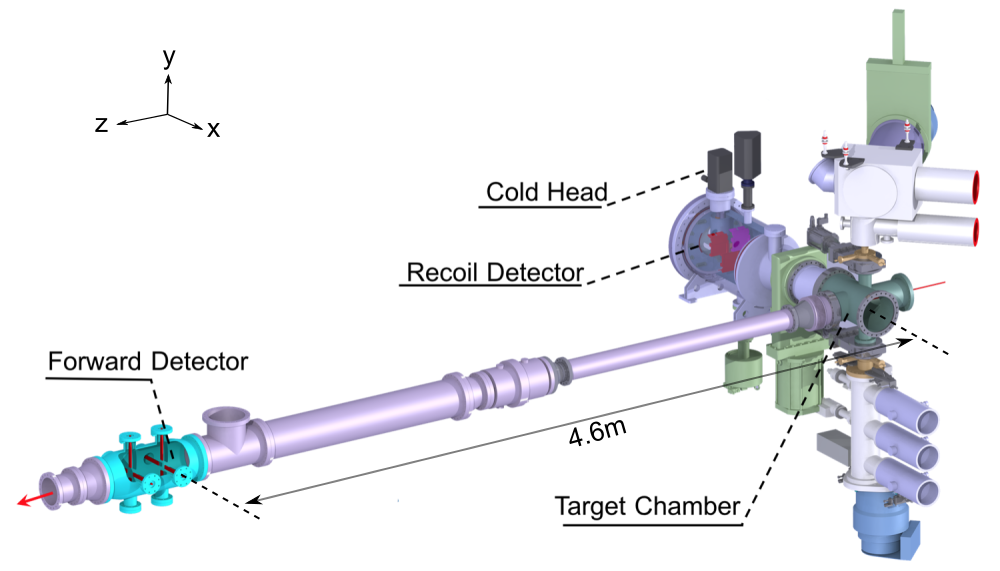
\includegraphics[width=0.8\textwidth]{./koala_setup.png}
	\caption{3D visualization of KOALA setup at COSY}
	\label{fig:setup}
\end{figure*}

The KOALA experiment is a fixed-target experiment aiming to measure the
differential cross-section of $\bar{p}p$ or $pp$ elastic scattering
over the four-momentum transfer range $0.0008 < |t| < \SI{0.1}{\tmom}$, which
covers the CNI region.
Due to the identical kinematics of $\bar{p}p$ and $pp$ elastic scattering, the
same setup of KOALA can be used in both measurements.
It is scheduled to measure $\bar{p}p$ elastic
scattering at the future HESR ring of FAIR \cite{FAIR} in the beam momentum range from
\SIrange{1.5}{15}{\momentum}.
Before the commission of HESR, KOALA is scheduled to be ran at COSY \cite{COSY}
for measuring $pp$ elastic scattering in the beam momentum range from \SIrange{1.5}{3.4}{\momentum}.
Over these beam energy range, KOALA covers the different regions where the Coulomb interaction, the CNI and the nuclear interaction are all significant.
The so called Coulomb normalization method \cite{bernard1987real,jenni2008atlas} can be used once Coulomb region is reached.
This enables the possibility of the determination of \({\sigma}_{tot}\), \(b\), \(\rho\) as well as
the absolute luminosity by analyzing the characteristic shape of $dN/dt$
spectrum (i.e. relative differential cross section) \cite{recoil_article}.
The absolute differential cross section can be normalized accordingly.

Due to the limitation of beam pipe aperture and the beam emittance,
it is extremely difficult to measure the scattering particle over a wide range of scattering angle in the forward direction.
The recoil measurement technique ,which means precise measurement of both the recoil angle and the kinetic energy of the recoil proton, 
is used to determine the differential elastic scattering cross section in KOALA.
Identification of the elastic scattering events is based on the match between the recoil angle and the kinetic energy.
A recoil detector based on this idea has already been built and the method of recoil measurement technique was verified using proton beams at COSY \cite{recoil_article}.
However, it was found in these tests that the identification of elastic events was limited by the large contamination of low-energy
background events at small recoil angles, which correspond to $|t| < \SI{0.002}{\tmom}$.

% To reach the remaining range \(0.0008 < |t| < 0.001\) \((GeV/c)^2\) in KOALA, a coincidence measurement between the recoil proton and scattering beam particle is proposed to suppress the background contamination.
% A time-sensing forward detector with a limited coverage range at small scattering angle is designed and built for this purpose. 
% the coincidence measurement between the recoil proton and scattering beam particle is proposed.
The low-energy backgrounds are mainly from inelastic scattering processes.
In order to suppress them and achieve the designed $|t|$-range, a forward detector based on fast-timing plastic scintillator is
employed to measure the elastically scattered beam particle near the beam axis.
This full setup of KOALA , consisting of the recoil detector, the newly-built forward detector and other upgraded components,  are installed at COSY.
Several tests using proton beams have been carried out to verify the design and the performance.
In the following sections,  the full system of KOALA at COSY is described and the preliminary results from the beam tests are presented.

\section{Experimental setup at COSY}
\label{sec:setup}

KOALA is installed at a linear section in the COSY ring.
The setup consists of three arms as shown in Fig. \ref{fig:setup}: the hydrogen
cluster target arm, the recoil arm and the forward arm.
All components inside these arms are installed in the same vacuum space as the beam.

The hydrogen cluster target connects vertically to the target chamber, with the target generator on the top and the target beam dump on the bottom.
The recoil arm is oriented along -X axis of the laboratory frame.
The chamber holding the recoil detector sensors are separated with target
chamber with a vacuum gate valve.
This valve is used for staged pumping of the recoil chamber during the
preparation of the experiment and protects the recoil sensors from the residual
gas inside the beam pipe.
The forward chamber locates about \SI{4.6}{\meter} away from the target center and
connects to the target chamber through two beam pipes with the diameter \SI{90}{\mm} and \SI{200}{\mm} respectively. 

\subsection{Hydrogen cluster target}
\label{sec:target}

A thin hydrogen cluster target, which can be operated under ultra high vacuum
environment, is critical for the sucess of KOALA.
First, the energy loss of recoil proton before hitting the recoil sensor should
be minimized so that an accurate determination of its kinetic energy is possible.
Second, the thickness of the target (i.e. the profile along the beam direction) determines
the spread of the vertex distribution of beam-target interaction.
Since there is no tracking device in KOALA, the spread will deteriorate the
angular resolution as well as the energy spectrum shape.

The hydrogen cluster target, which was used previously in ANKE experiment
\cite{cluster_target}, is upgraded in KOALA.
A special collimator is built to achieve a much
smaller width of the cluster along the beam axis.
The target thickness in terms of full width at half maximum (FWHM) is measured
to be $\sim\SI{1.5}{\mm}$ close to the interaction point (IP).
The areal density is estimated to be \SI{e14}{\atom\per\cm\squared}.

\subsection{Recoil detector}
\label{sec:recoil}

The recoil detector needs to totally stop the recoil proton from the
elastic scattering and measure its total kinetic energy.
For elastic scattering of two particles with the same mass,
the kinetic energy of recoil proton \(T_p\) is proportional to four-momentum
transfer squared by \(|t| = 2m_pT_p\), where \(m_p\) is the proton mass.
For the maximum $|t|=\SI{0.1}{\tmom}$, \(T_p \approx \SI{54}{\MeV}\). Thus, a dynamic range of
$0\sim\SI{60}{\MeV}$ is required of the recoil detector.

\begin{figure}[htbp]
  \centering
  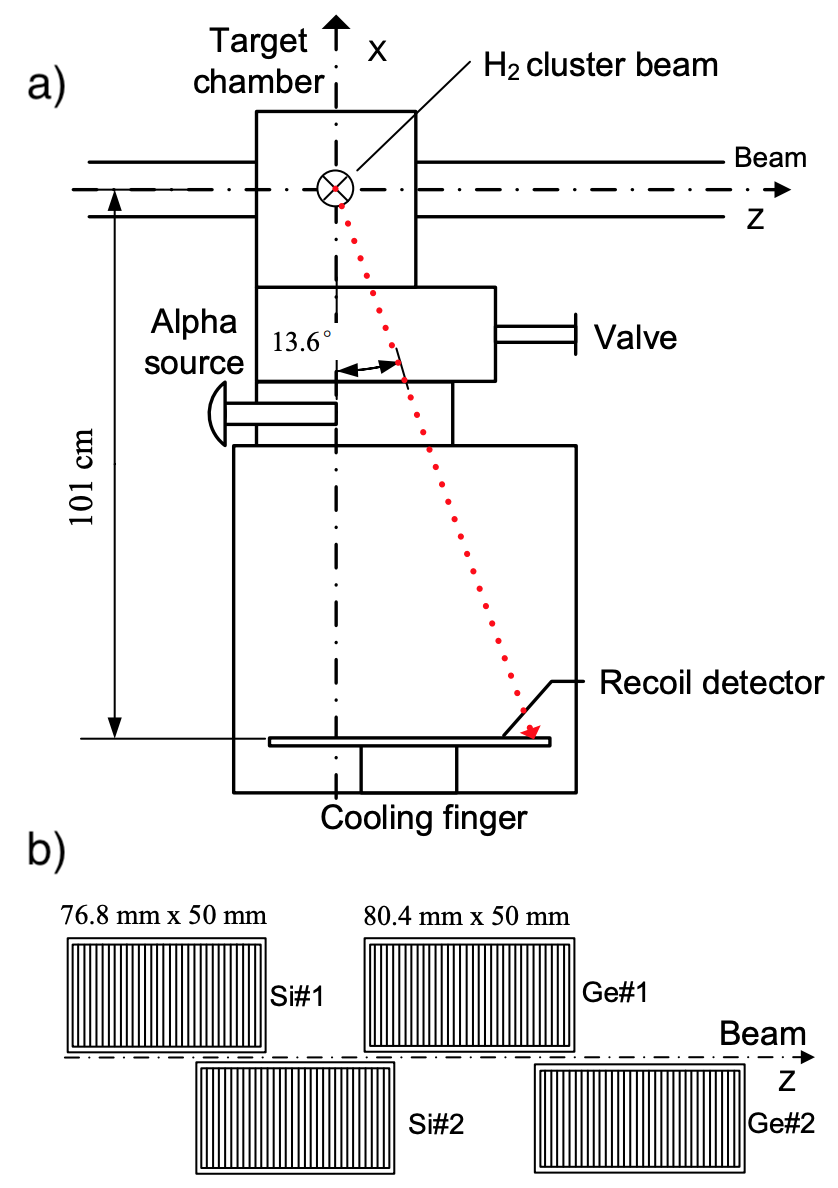
\includegraphics[width=0.4\textwidth]{./recoil_schematic.png}
  \caption{(a) Schematic view of the recoil detector configuration, seen from the
    top; (b) Layout of the four recoil sensors, seen from +X direction}
  \label{fig:recoil_schematic}
\end{figure}

The recoil detector consists of two single-sided silicon strip sensors and two
single-sided germanium strip sensors with a layout shown in Fig. \ref{fig:recoil_schematic}.
The detector plane is installed \SI{90.4}{\cm} away from the beam-target center
and covers a range of recoil angle $\SI{-1.5}{\degree} < \alpha < \SI{15}{\degree}$.
The sensors are arranged along the beam axis with staggered placement in the Y-axis.
Sensors at different recoil angle have different thickness: \SI{1}{\mm} for Si1
and Si2, \SI{5}{\mm} for Ge1 and \SI{11}{\mm} for Ge2.
The silicon sensors have an sensitive area of $76.8 \times \SI{50}{\mm\squared}$, which are
segmented into 64 strips of \SI{1.2}{\mm} pitch.
The germanium sensors have an sensitive area of \(80.4 \times \SI{50}{\mm\squared}\), which are segmented into 67 strips of \SI{1.2}{\mm} pitch.
This gives an angular resolution of about \SI{0.08}{\degree}.
By design, neighboring sensors have an overlapping region which is symmetric against
the beam axis (20 strips for Si1/Si2 overlapping, 9 strips for Si2/Ge1 overlapping, 10 strips for Ge1/Ge2 overlapping).
The overlapping strips are used for the correction of beam position asymmetry.

The recoil sensors are read out by a combination of the charge-sensitive preamplifier (MPR16 for the strips, MPR1 for the rear side) 
and the timing filter amplifier (MSCF16), all from Mesytec \cite{mesytec}. 
MSCF16 integrates the shaping amplifier and the leading edge discriminator in the same module.
Both amplitude and timing signal are extracted from MSCF16 for energy and time measurement.
% Strips at larger recoil angles are read out by a single channel without sacrificing the angular resolution.
In total, there are 180 readout channels for the recoil detector: 
48 channels on Si1, 64 channels on Si2, 32 channels for Ge1 and Ge2 and 4
channels for the rear sides. 

Soild-state sensors (especially germanium) need low and stable operating temperature to optimize energy
resolution.
Temperature of the recoil sensors are monitored by four temperature sensors
attached to the detector holder.
The operating temperature can be actively adjusted by a combination of a cold head and two heating resistors on the cold plate.
A study of the performance of recoil sensors in the laboratory shows that the
optimal working temperature of the recoil detector is \SI{125}{\kelvin}.
Under this condition, the energy resolutions of the silicon and germanium
sensors are better than \SI{20}{\keV} and \SI{30}{\keV} (FWHM) respectively.

$\alpha$ sources for the energy calibration are also installed inside the recoil chamber and fixed on a linear motion feedthrough rod.
During experiment, the rod is lifted and the sources are blocked by the chamber wall;
when calibration is needed, the rod is pushed to the chamber center and the sources face the recoil sensors directly.
Thus, the recoil detector can be calibrated regularly when no beam is circulating.

More technical information and the detailed performance tests of the recoil detector can be found in \cite{recoil_article}.

\subsection{Forward detector}
\label{sec:fwd}

% The forward detector aims to detect the elastically scattered beam proton in the
% forward direction and measure its arrival time.

The forward detector consists of 8 detector modules, which are
grouped into 4 pairs as shown in Fig. \ref{fig:setup}.
They are installed symmetrically on +X, -X, +Y and -Y axis, with the same
distance of \SI{3}{\cm} away from the beam pipe center.
The first layer of each pair are installed \SI{4.6}{\meter} away from the
beam-target center, and the seperation between the two layer is \SI{20}{\cm}.
Only the pair on +X is used for the conincidence measurement with the recoil detector.
The other 3 pairs are used for beam position tuning during beam preparation and
monitoring during the experiment.

Each detector module is made of plastic scintillator BC-408 \cite{bc408} with the dimension $90 (length) \times 20 (width) \times 6
(thickness)\,\si{\mm\tothe{3}}$.
% This corresponds to an angular acceptance of $\SI{0.37}{\degree} < \theta < \SI{1.49}{\degree}$.
The length of the scintillator guarantees the required coverage
from \SI{0.0008}{\tmom} to \SI{0.001}{\tmom} longitudinally over the COSY energy range.
However, the cross-sectional coverage, \textit{i.e.}, the coverage of the full length of
the recoil detector strips, depends not only on the beam energy but also on the
size of beam profile.
Fig. \ref{fig:forward_acceptance} shows an example of the impact of beam emittance on the
effective cross-sectional coverage.
The fully-covered area on the recoil detector shrinks with the increasing of beam emittance. 
\begin{figure}[htbp]
  \centering
  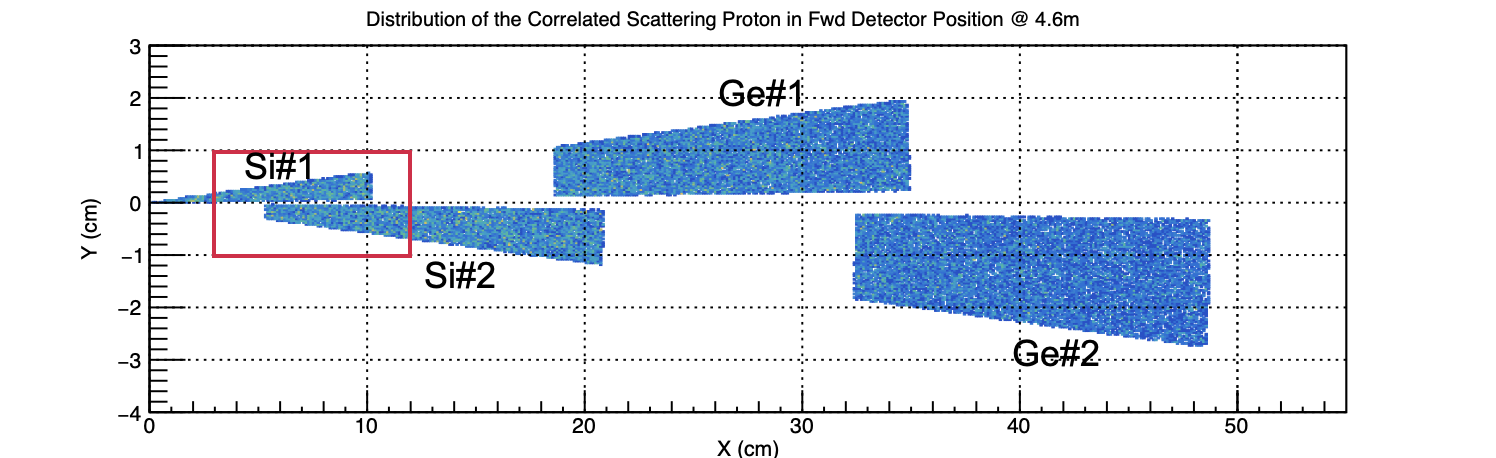
\includegraphics[width=0.45\textwidth]{./fwd_acceptance.png}
  \caption{
    Hit position distribution of the elastically scattered proton on the X-Y plane at \SI{4.6}{\meter}
    from the beam-target center. The results are from the simulation of \SI{2.2}{\momentum}
    $pp$ elasitc scattering with an uniform spherical distribution in the
    center-of-mass reference frame: up) ideal point beam; down) $\SI{10}{\mm}\times\SI{10}{\mm}$ box beam profile.
    % for the elastic scattering events in which
    % the recoil proton hits one of the recoil sensors.
    The four blue blocks are from the events in which the recoil proton hits one of
    the four recoil sensors.
    The red square indicates the dimension of the forward detector scintillator
    and the vertical dashed line indicates the hit position when $|t| = \SI{0.001}{\tmom}$.}
  \label{fig:forward_acceptance}
\end{figure}
Based simulation study, the current width of the forward detector scintillator guarantees the
full cross-sectional coverage for $|t| < \SI{0.001}{\tmom}$ as long as the beam profile size is smaller than \SI{7}{\mm}.
The actual coverage can to be extracted in the data analyis, see Sec. \ref{sec:result}.

The scintillator is readout by the combination of a tapered light guide, a piece of silicone pad and a
photomultiplier tube (Hamamastu H6900 \cite{hamamatsu}), as shown in Fig. \ref{fig:forward_module} (a).
Each detector module is integrated with a forward chamber flange for the usage
in the ultra-high vacuum environment.
To protect the vacuum condition inside the beam pipe, the following designs are implemented:
\begin{enumerate}
\item only the light guide and the scintillator are installed inside the forward chamber, the light guide is glued on the open port of the flange as a feedthrough;
\item no wrapping and painting material on the surface of the scintillator, the surface is polished to increase light collection efficiency;
\item a thin aluminum tube with thickness of \SI{100}{\micro\meter} is used as
  the light shield to prevent the light cross-talk between scintillators, the tube is screwed on the flange, see Fig. \ref{fig:forward_module} (b);
\item two small holes are opened on the wall of the aluminum tube to speed up vacuum pumping, see Fig. \ref{fig:forward_module} (c).
\end{enumerate}
Other components like the silicone pad, the PMT and the PMT base are installed inside a light-tight case on the other side of the flange as shown in Fig. \ref{fig:forward_module} (c).
\begin{figure}[htbp]
  \centering
  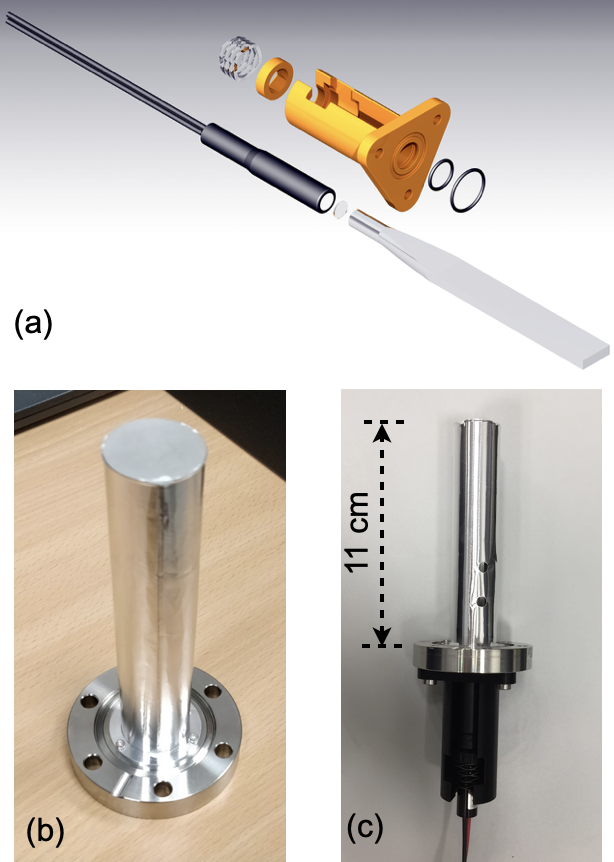
\includegraphics[width=0.32\textwidth]{./forward_module.png}
  \caption{(a) CAD model of the assembly of forward detector module; (b) The aluminum tube is fixed on the inside of the flange; (c) One forward detector module after complete assembly}
  \label{fig:forward_module}
\end{figure}
% \begin{figure}[htbp]
%   \centering
%   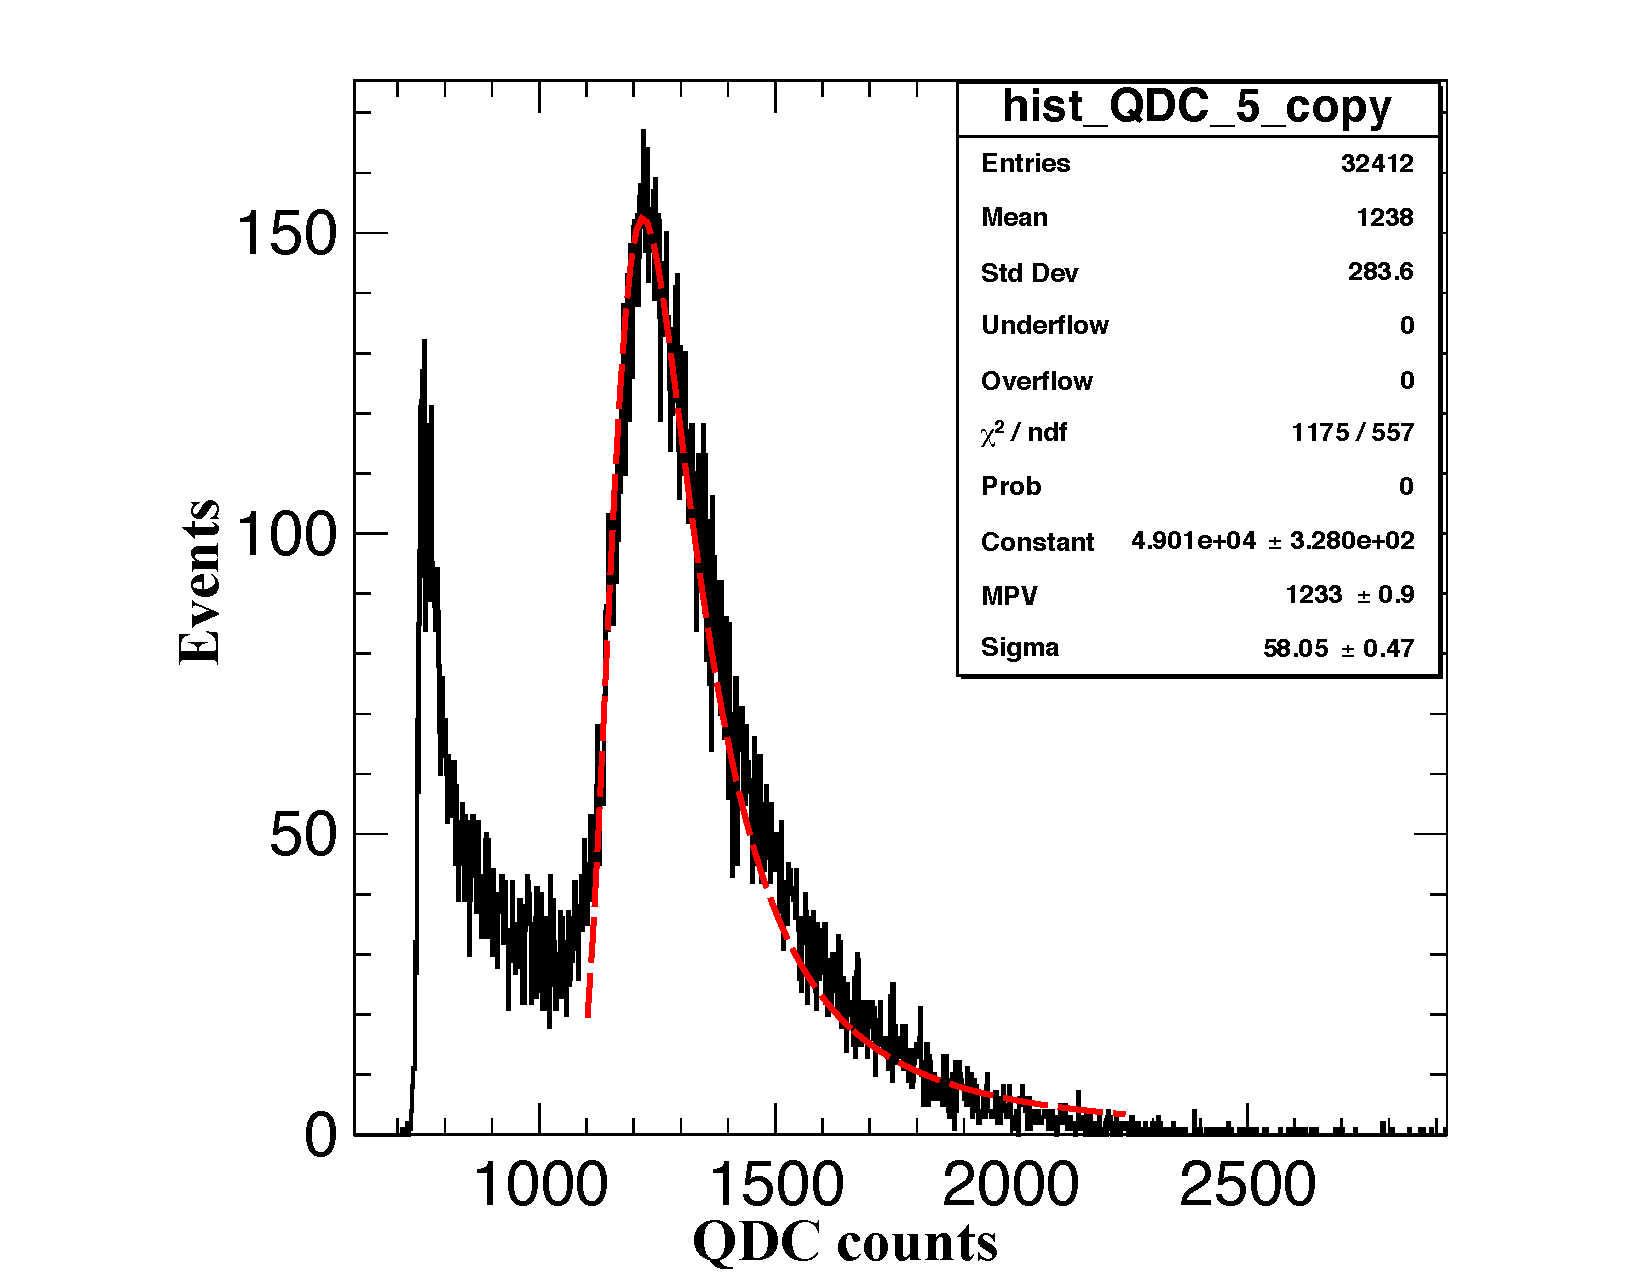
\includegraphics[width=0.4\textwidth]{./forward_mip.pdf}
%   \caption{An example of the cosmic ray energy spectrum obtained by a forward detector module}
%   \label{fig:forward_mip}
% \end{figure}

Due to the large gain of PMT, no front-end electronics is needed for the readout of the forward detector.
The output signal from H6900 is split into two branches: one fed to a
constant fraction discriminator for time information extraction; the other for charge measurement directly.
Modules are tested using cosmic ray in laboratory before installation.
% A typical MIP spectrum obtained by the forward detector module is shown in Fig. \ref{fig:forward_mip}. 
The peak of minimum ionizing particle (MIP) is well separated from the pedestal
noise, with the signal to noise ratio (SNR)larger than 50.
The timing resolution is measured to be about \SI{140}{\pico\second}.

\begin{figure*}[htbp]
  \centering
  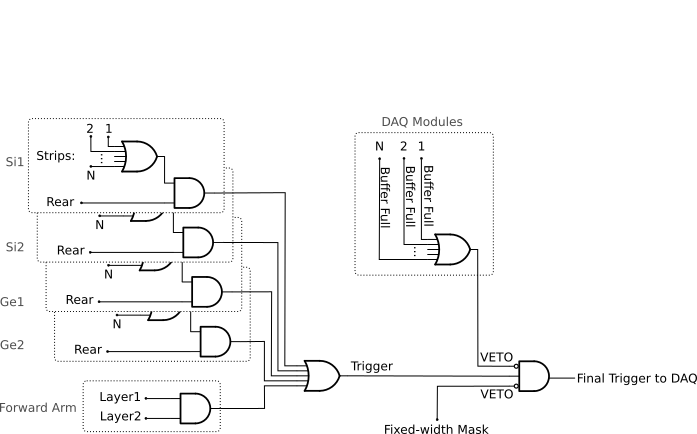
\includegraphics[width=0.75\textwidth]{./trigger_logic.png}
  \caption{Trigger Logic of the KOALA DAQ.}
  \label{fig:trigger_logic}
\end{figure*}

\section{Data acquisition system}
\label{sec:daq}

The data acquisition system of KOALA is a VME-based system with multiple types
of digitization modules produced by Mesytec \cite{mesytec}.
For the recoil detector, the amplitude signal from MSCF16 is digitized by a
peak-sensing ADC module MADC-32.
MADC-32 has a 13-bit dynamic range with \SI{6.4}{\micro\second} conversion time.
For the forward detector, the pulses from PMTs are directly fed into a QDC
module MQDC-32 for the charge measurement.
MQDC-32 has a dynamic range of \SI{500}{\pico\coulomb} with 12-bit resolution
and \SI{250}{\nano\second} conversion time.
The timing information from both the recoil and forward detectors are recorded by a TDC module MTDC-32 using the conventional Start-Stop method.
MTDC-32 has a minimum resolution of \SI{4}{\pico\second} and
\SI{32}{\pico\second} is used for the forward detector.
A multi-channel scalar SIS3820 \cite{sis} is also integrated to record
the following key count rates: 1) count rates of the four pairs of the forward detector for beam position monitoring; 2) count rates of the overlapping regions of the recoil detector for asymmetry correction; 3) count rates of the input trigger
for DAQ efficiency correction.

% The acceptance of the forward detector only covers a small part of the recoil detector sensors.
% To record the elastic scattering events from the whole range of the recoil angle
% covered by the recoil detector,
KOALA adopts a self-triggering scheme for the trigger logic design.
Each sensor of the recoil detector and +X arm of the forward detector works independently and generates their own trigger. 
The final trigger to the DAQ is a common OR of all sub-detectors, as shown in Fig. \ref{fig:trigger_logic}.
The trigger from the recoil detector sensor is generated by a coincidence between the front-side strips and the rear-side plane, 
and the trigger from the forward detector arm is generated by a coincidence between the two modules in the same pair.
% In this way, the rate of the false hits generated by electronic noise can be minimized.
Both elastic and inelastic scattering events are recorded in this trigger design, and the coincidence between the recoil sensor and the forward detector is carried out in offline analysis.

Fast readout of the recorded event is crucial for a self-triggered DAQ system.
The asynchronous readout mechanism combined with VME CBLT block read mode is adopted to increase the data throughput in KOALA.
The digitization modules used in KOALA all have an event buffer with a size
larger than \SI{32}{\kilo\byte}.
Digitized events are stored in this buffer before readout, so that the module is immediately available to digitize the next event.
Events will not be readout until the buffer is nearly full.
On the other hand, since the cross section is much higher at smaller recoil
angle, the module buffer for these channels always saturates faster than others.
These modules may miss new coming events while others not, and thus bringing a systematic bias.
To overcome this issue, the buffer-full signal from each module is added to the trigger logic as \texttt{VETO} as shown in Fig. \ref{fig:trigger_logic}.

The issue about event synchronization arises naturally when using asynchronous
readout mode.
% The digitization modules used in KOALA have different dead time, especially between MADC-32 and MTDC-32.
% An event recorded by a fast module may be missed by a slow module. This creates un-synchronous event structure, which makes the sequential event data assembling impossible. 
Timestamp-based synchronization is used to solve this problem.
The modules in the system have a 30-bit counter for recording the timestamp from
the clock signal distributed by a central source.
The source could be either the VME built-in clock (\SI{16}{\MHz}) or an external clock
(lower than \SI{75}{\MHz}).
Currently, the built-in clock of VME backplane bus is used. 
Based on this timestamp, event synchronization is achieved offline.
The other option is adding a fixed-width mask gate into the trigger logic as \texttt{VETO}, see Fig. \ref{fig:trigger_logic}.
The width of the mask gate should be larger than the maximum dead time of all modules.
In this way, the events are effectively synchronized sequentially. 
However, this method may reduce DAQ efficiency significantly in a high hit-rate environment.

\begin{figure}[htbp]
\centering
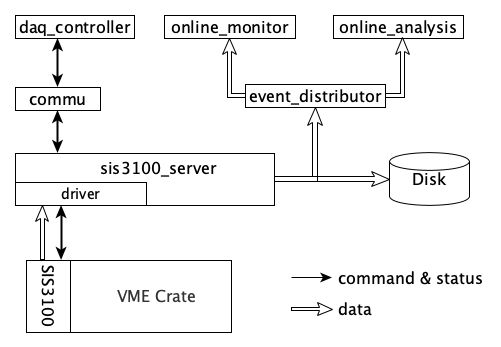
\includegraphics[width=0.45\textwidth]{./koalaems_deployment.png}
\caption{Design and deployment of KoalaEms.}
\label{fig:koalaems}
\end{figure}

% \raggedright
A dedicated DAQ software called KoalaEms is also developed for KOALA.
KoalaEms is a fork of the EMS software \cite{ems}, which is a highly flexible DAQ software framework developed for various experiments at COSY.
Support for the VME controller (SIS3100 \cite{sis}) is integrated and a new component of online monitoring based on ROOT is added.
The architecture of KoalaEms is shown in Fig. \ref{fig:koalaems}.
The interface to the DAQ is implemented as \linebreak\texttt{sis3100\textunderscore server}, the host of which
connects to SIS3100 by an optical link.
The control and status information from/to the GUI \texttt{daq\textunderscore controller} is mediated by a component called \texttt{commu}.
The data flow from VME crate is split into two branches: 1) \texttt{data\textunderscore out\textunderscore disk}: save the raw data onto disk; 2) \texttt{data\textunderscore out\textunderscore stream}: stream out to \texttt{event\textunderscore distributor}.
\texttt{event\textunderscore distributor} will forward the data stream to various consumption hosts for usages like online monitoring and online analysis.
Both \texttt{commu} and \texttt{event\textunderscore distributor} support socket connection and the \texttt{event\textunderscore distributor} also supports multiplexing streaming.
All components shown in Fig. \ref{fig:koalaems} can be hosted in different PC and new consumption host to the data stream can be integrated whenever needed.
% \justify

\section{Software framework}
\label{sec:software}

A software framework called KoalaSoft is developped for the simulation, calibration, reconstruction and analysis jobs of the KOALA experiment.
It is built upon the FairRoot \cite{fairroot} framework, which implements a simulation environment based on VMC \cite{vmc} library and an analysis environment based on ROOT's task concept.
The components stack of KoalaSoft is shown in Fig. \ref{fig:koalasoft}.

\begin{figure}[htbp]
  \centering
  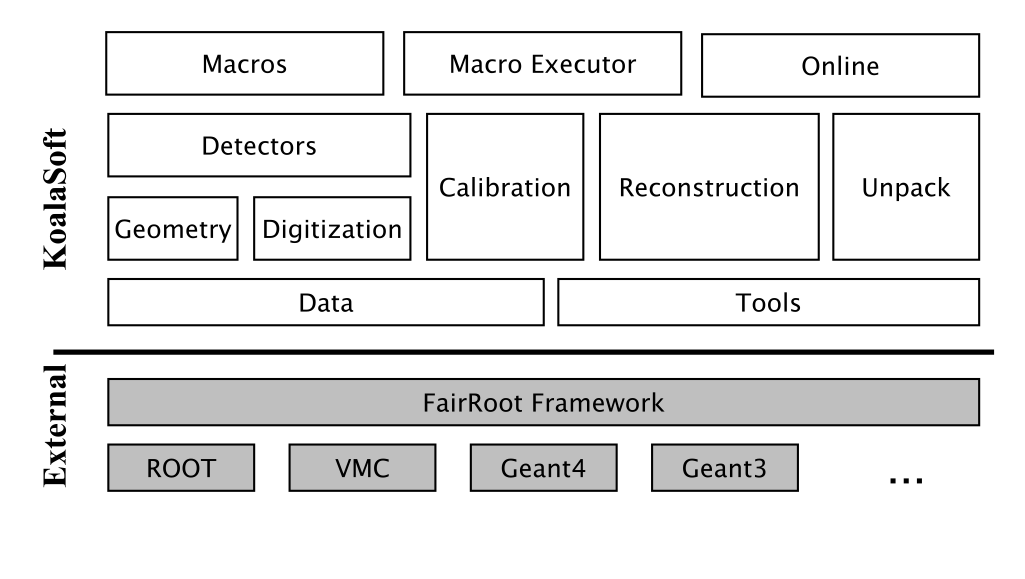
\includegraphics[width=0.48\textwidth]{./koalasoft_components.png}
  \caption{Components of KoalaSoft}
  \label{fig:koalasoft}
\end{figure}

Both Geant3 and Geant4 can be selected as the simulation engine without changing other components in KoalaSoft.
Geometry models of the recoil detector and the forward detector are implemented using ROOT's TGeo library.
Jobs like digitization, calibration and reconstruction are divided into multiple smaller steps, each of which is represented by a single task.
Tasks chained together later in a ROOT macro to compose a full job. 
ROOT macros are the interface for the end user using KoalaSoft.
Macros for common jobs are pre-configured and distributed along with KoalaSoft.
Users can also compose their own specific jobs for analysis.
Additionally, a binary macro executor is provided to run jobs directly from command line. This may be useful in batch processing.

The same chain of tasks can be used for the analysis of both the simulation data and the raw data from DAQ.
This is accomplished by the \texttt{Unpack} component, which can decode and transform the raw binary data into the same format as the output from simulation jobs.
Thus, algorithms developped, tested and verified using simulation data can be applied to experimental data seamlessly.
This saves a lot of efforts in the development and maintainence of algorithms.
Both the offline disk data and the online streaming data are correctly handled by \texttt{Unpack} and an online monitoring program is developped based on it.

\section{Reconstruction}
\label{sec:reconstruction}

\subsection{Energy calibration}
\label{sec:calibration}

% Precise measurement of energy deposit in the recoil detector is critical for the
% identification of elastic scattering events as well as the calculation of the recoil angle.
\(^{239}Pu\), \(^{244}Cm\), \(^{241}Am\), with main $\alpha$ decay energies
of \SIlist{5156.59;5804.83;5485.56}{\keV} \cite{nuclear_data} respectively, are
used for the energy calibration of the recoil detector.
Decays with smaller branch ratios are also utilized if they are well separated from the main peaks.

Two aspects need special consideration in the calibration.
First, the recoil sensors have a thin protective layer on the surface and this
causes energy loss before particles enter the fiducial volume of the sensor.
The thickness of the protection layer has been measured in the laboratory using \(\gamma\) rays \cite{recoil_article}
and corresponding enery loss of $\alpha$ particles can be estimated with
LISE++ program \cite{LISE}.
The estimated energy loss at normal incidence angle are listed in Tab.
\ref{tab:dead_layer} for each sensor.
The effective energy deposit in the fiducial volume is then corrected based on the recoil angle, where each strip is located.

\begin{table}[htbp]
\label{tab:dead_layer}
\caption{Energy loss of $\alpha$ in the protection layer (\SI{90}{\degree})}
\centering
\begin{tabular}{cccccc}
\hline
\(E_{\alpha} (keV)\) & \(\Delta E_{Si1}\) & \(\Delta E_{Si2}\) & \(\Delta E_{Ge1}\) & \(\Delta E_{Ge2}\) \\
\hline
5156.59 & 11.51 & 11.51 & 110.00 & 111.00 \\
5485.56 & 11.01 & 11.01 & 105.00 & 106.00 \\
5804.83 & 10.52 & 10.52 & 99.00  & 100.00 \\
\hline
\end{tabular}
\end{table}

Secondly, the gain setting of each readout channel is optimized for the energy range covered by the corresponding strip.
The gain difference varies up to a factor $\mathtt{\sim}$10.
Thus, the resolution is worse at large recoil angle than at small angle, as shown in Fig. \ref{fig:alpha_spectrum}.
The minor decay modes can't be recognized in Fig. \ref{fig:alpha_spectrum} (a), while they are clearly seen in Fig. \ref{fig:alpha_spectrum} (b).
Lower resolution brings larger uncerntainty in the calibration, since only three energy points can be used.
\begin{figure*}[htb!]
  \centering
  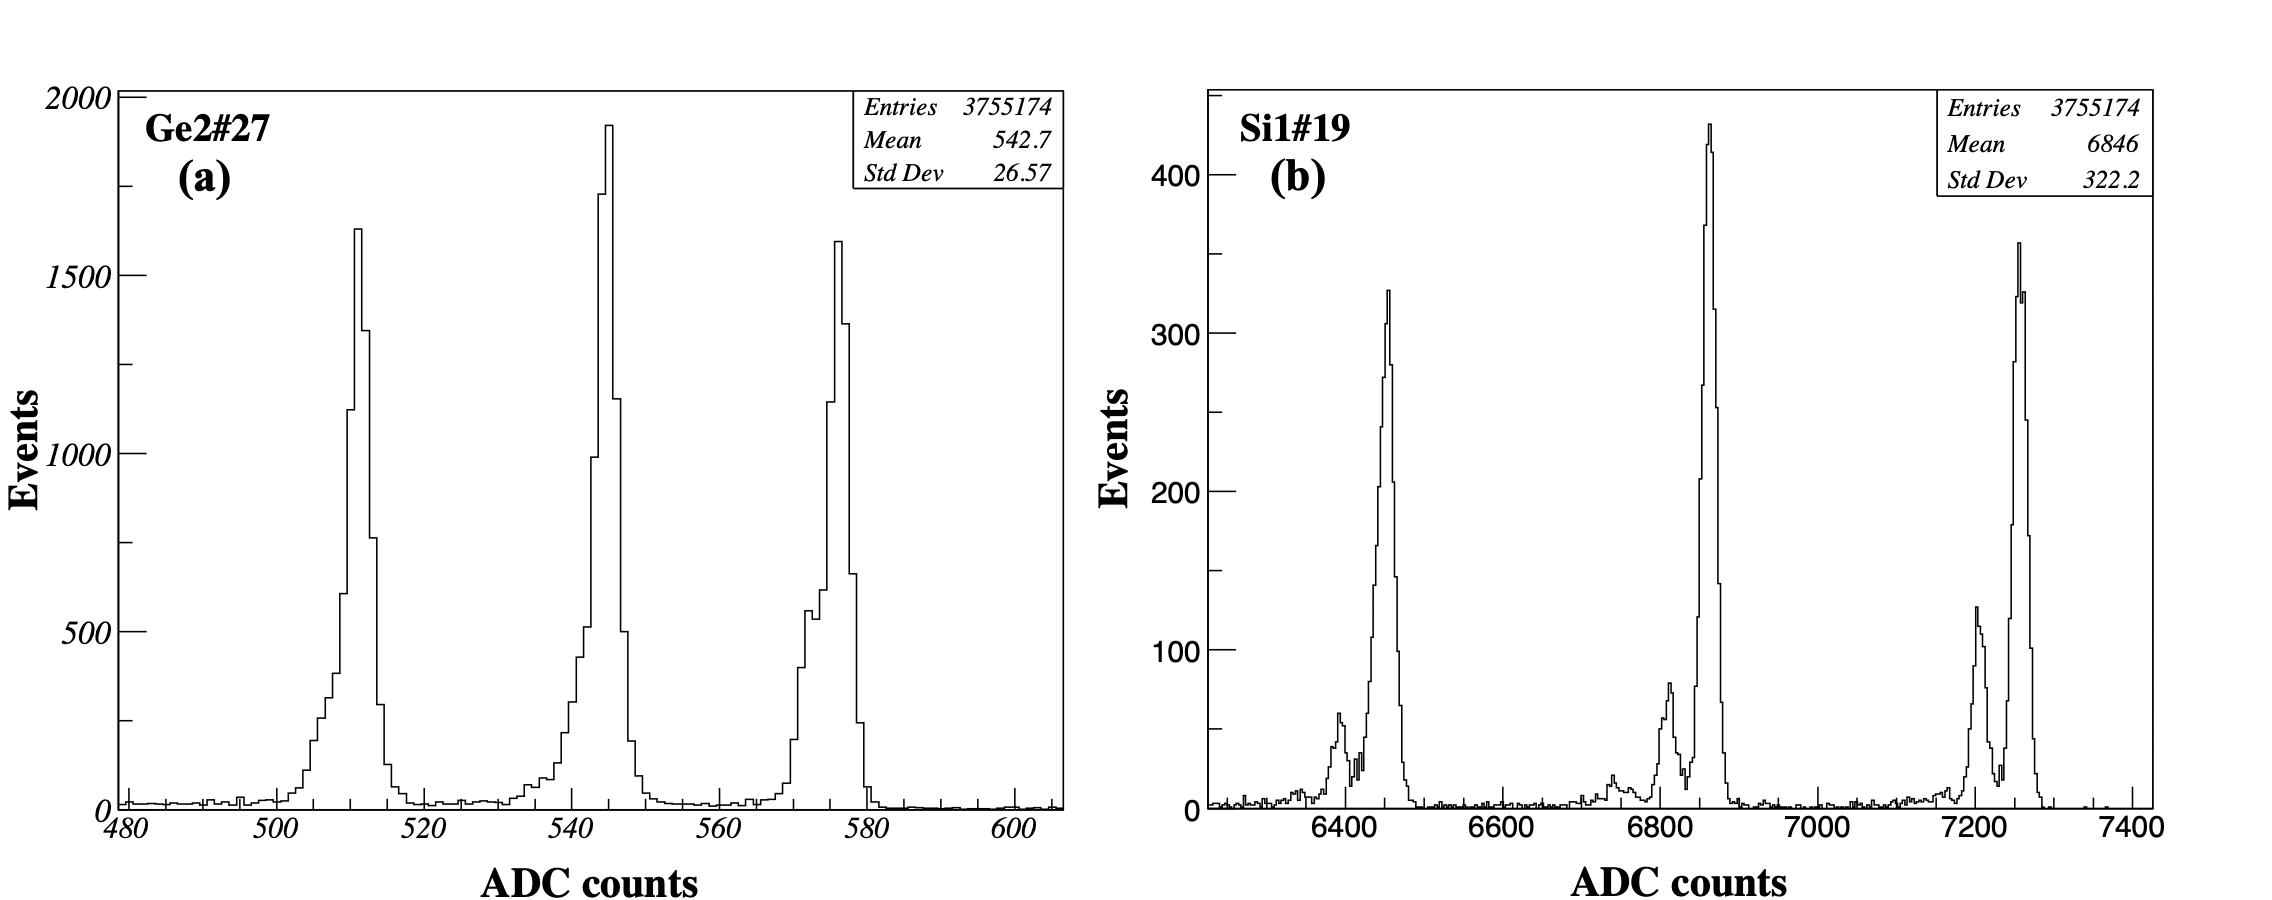
\includegraphics[width=0.7\textwidth]{./alpha_response.png}
  \caption{Example energy spectra of \(\alpha\) sources of two channels at different positions: (a) large recoil angle $13.9\degree$; (b) small recoil angle $0.93\degree$}
  \label{fig:alpha_spectrum}
\end{figure*}

To minimize this uncerntainty, a common gain setting, which is optimized for the separation of the \(\alpha\) peaks, is set for all channels.
The calibration is carried out indirectly as follows:
\begin{enumerate}
\item \(\alpha\) source calibration is carried out under the common gain setting;
\item the linearity curves at both the common gain and the so-called beam gain used
  in experiment are calibrated using a precision pulse generator (ORTEC Model 419);
\item the $\alpha$ peak at the beam gain is then deduced
  from the linearity curve at a pulser amplitude, which generates the same peak
  value as the $\alpha$ source at the common gain;
\item the peak responses are fitted linearly against the corresponding $\alpha$ energies
  to get the calibration parameters.
\end{enumerate}
The readout electronics of the recoil detector has very good linearity in both
common gain and beam gain setting (see Fig. \ref{fig:electronic_linearity}),
thus linear fitting is adopted in all the calibration steps.
% Due to the good linearity of the readout electronics in both common gain
% and beam gain setting (see Fig. \ref{fig:electronic_linearity}), this indirect
% method does not bring in extra systematic bias.
The fitting parameters from the last step are used to convert ADC counts into
energy values in the reconstruction.
% The achieved precsion of the calibration is about \SI{0.12}{\percent}.
\begin{figure}[htb!]
  \centering
  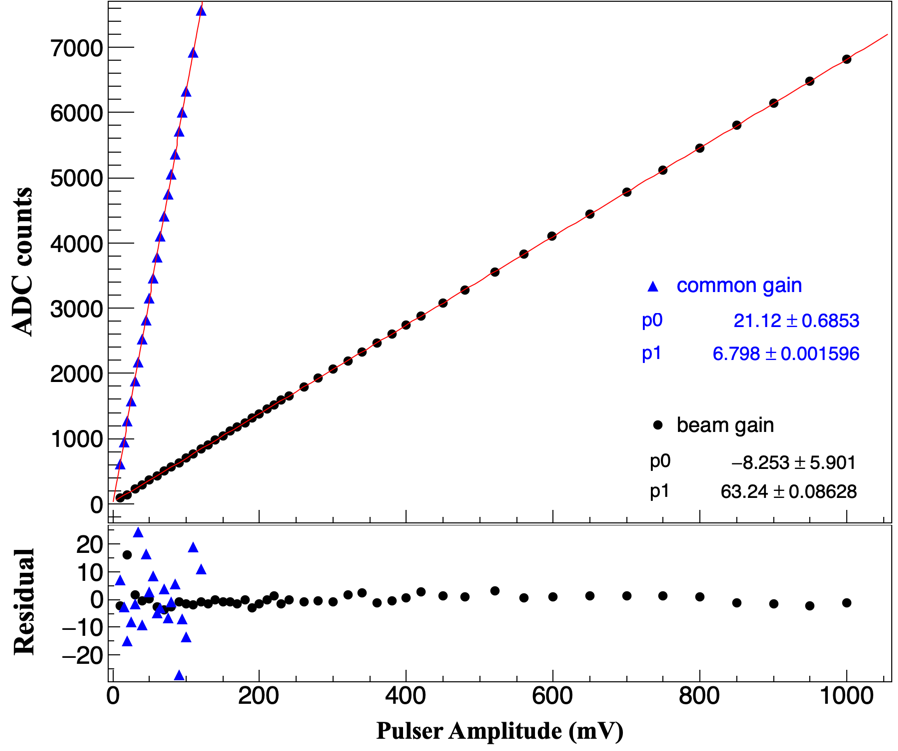
\includegraphics[width=0.42\textwidth]{./linearity.png}
  \caption{Electronic linearity of a typical recoil detector channel}
  \label{fig:electronic_linearity}
\end{figure}

\subsection{Time walk correction}
\label{sec:timewalk}

Time walk of the leading edge discriminator used in the recoil detector needs to be corrected to
optimize the timing resoultion.
The calibration of the time-walk effect is carried out with ORTEC Model 419. 
Output of the pulser is split into two branches: one is fed into a constant fraction discriminator to generate the reference time;
the other is connected to the detector channel under calibration for the time measurment. 
By scanning the pulser over a wide range of amplitudes, the time-walk effect is revealed.
An example is shown in Fig. \ref{fig:timewalk}, where the result is fitted with \(y=p_0 x^{-1} + p_1\). 
The time walk is corrected by substracting \(\Delta t = p_0/ADC\) from the measured timing value.
\begin{figure}[htbp]
  \centering
  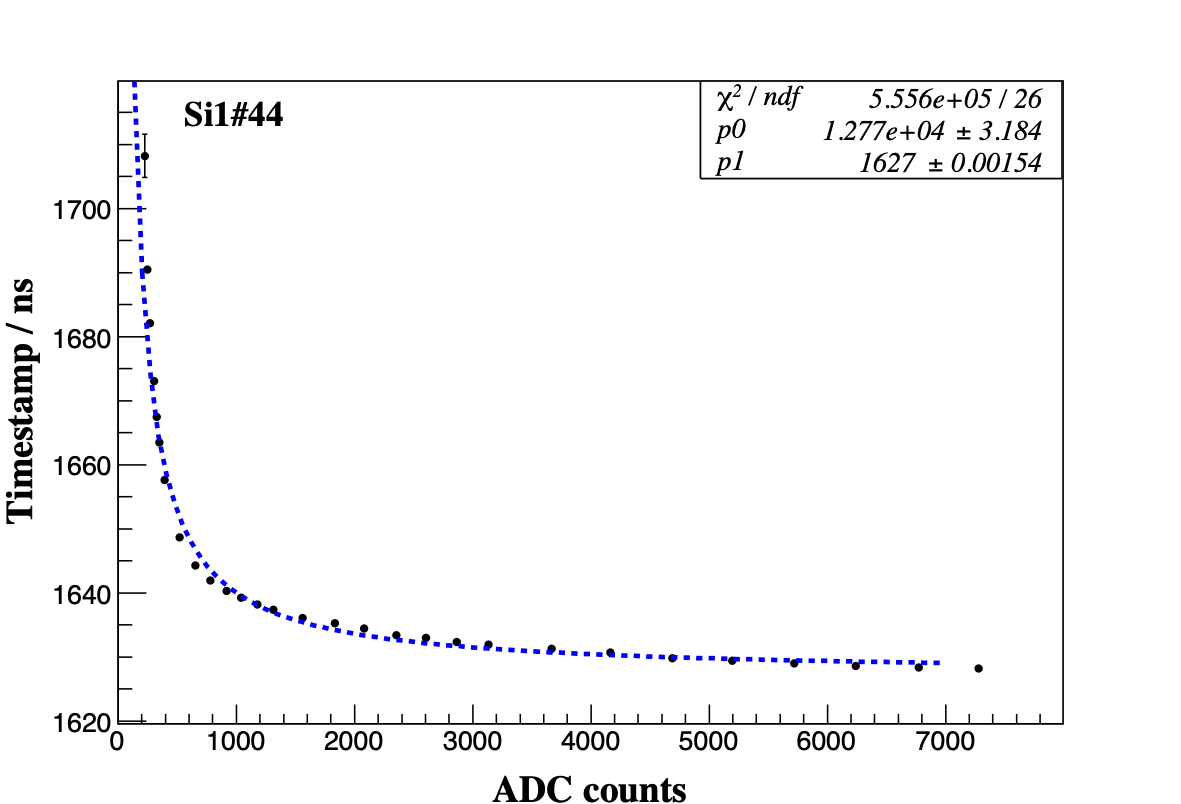
\includegraphics[width=0.45\textwidth]{./timewalk.png}
  \caption{Typical result from the time-walk calilbration.}
  \label{fig:timewalk}
\end{figure}

The difference of the fitting paramter \(p_1\) indicates the delay time
difference between different channels, which is caused by the signal routing length variation.
These offsets are also corrected in the reconstruction to align the timing from different channels.

\subsection{Clustering}
\label{clustering}

Clustering is necessary to reconstruct the correct energy deposit:
1) charge sharing is an intrinsic characteristic of the solid-state strip detector, especially
for the tracks hitting the region in between adjacent strips; 2) tracks with
large recoil angles may penetrate through several strips before stopping.
The results from the simulation and the beam commissioning both show that more than \SI{50}{\percent} of the tracks hitting Ge2 have hit multiplicity
larger than 1. The fractions of different hit multiplicities in the four
recoil sensors are listed in Tab. \ref{tab:multiplicity}.
% \begin{figure}[htbp]
%   \centering
%   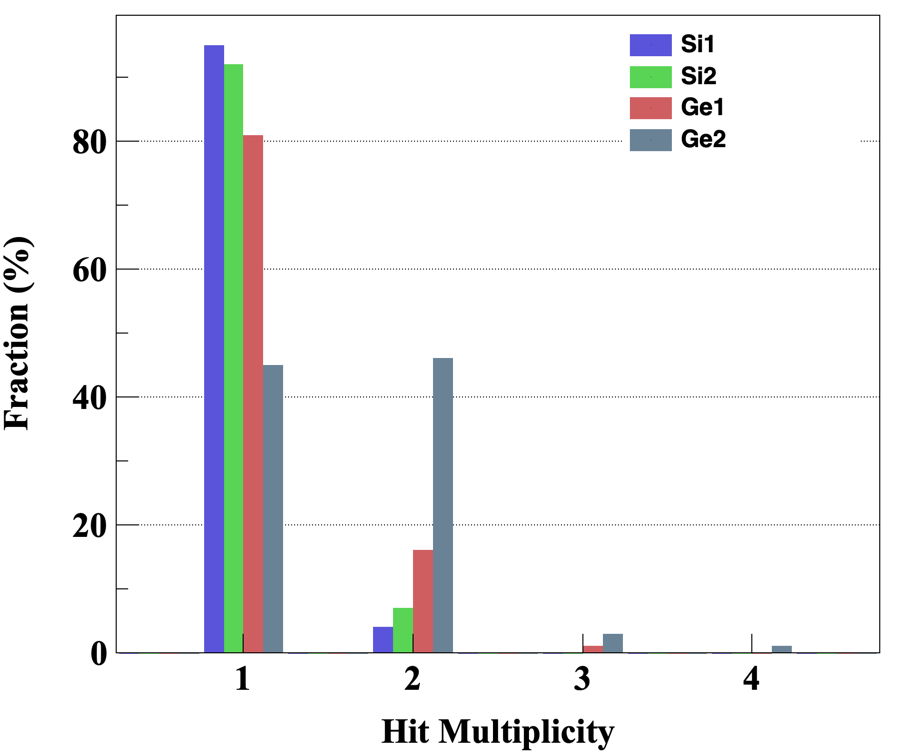
\includegraphics[width=0.45\textwidth]{./multiplicity.png}
%   \caption{Fraction of the hit multiplicity on each sensor of the recoil detector.}
%   \label{fig:multiplicity}
% \end{figure}

\begin{table}[htbp]
  \label{tab:multiplicity}
  \centering
  \caption{Hit multiplicity on the recoil detector at $P_{beam} = \SI{2.2}{\momentum}$}
  \begin{tabular}{cccccc}
    \hline
    Multiplicity (\si{\percent}) & 1& 2& 3&  4 \\
    \hline
    Si1 & 95.51 & 4.38 & 0.08 & 0.02 \\
    Si2 & 92.46 & 7.21 & 0.24 & 0.06 \\
    Ge1 & 81.06 & 16.61 & 1.51  & 0.44 \\
    Ge2 & 45.41 & 46.30 & 3.98  & 1.67 \\
    \hline
  \end{tabular}
\end{table}

The clustering algorithm is designed to minimize the noise contribution while
keeping the low-energy background characteristic as much as possible.
% It is also important not to bring a selection bias between low energy and high energy elastic events.
The steps of clustering in KOALA is as follows:
\begin{enumerate}
\item Delete noise hits. Hits induced by the electronic noise are deleted. A low
  threshold ($2\sigma_{noise}$) is used in this step.
\item Collect remaining hits into clusters based on the adjacency principle.
\item Delete noise clusters. The noise level of a cluster with $n$ hits is evaluated as
  $\sigma_{cluster} = \sqrt{\sum_{i=1}^n{(\sigma_{noise}^i)^2}}$, where $\sigma_{noise}^i$ is
  the noise level of $i$th strip in the cluster. Clusters which have
  energy lower than $5\sigma_{cluster}$ are considered to be noise-induced and deleted.
\item Delete clusters without seed hit. Valid cluster needs to have at lease one seed hit, the
  amplitude of which exceeds the equivalent energy of the trigger threshold of
  the corresponding strip.
\end{enumerate}
The hit position and hit time of the cluster are both extracted from the first
hit in the cluster to keep the most accurate information about the recoil angle.

The comparison between the energy spectrum before and after clustering is shown in
Fig. \ref{fig:clustering}.
\begin{figure}[h]
  \centering
  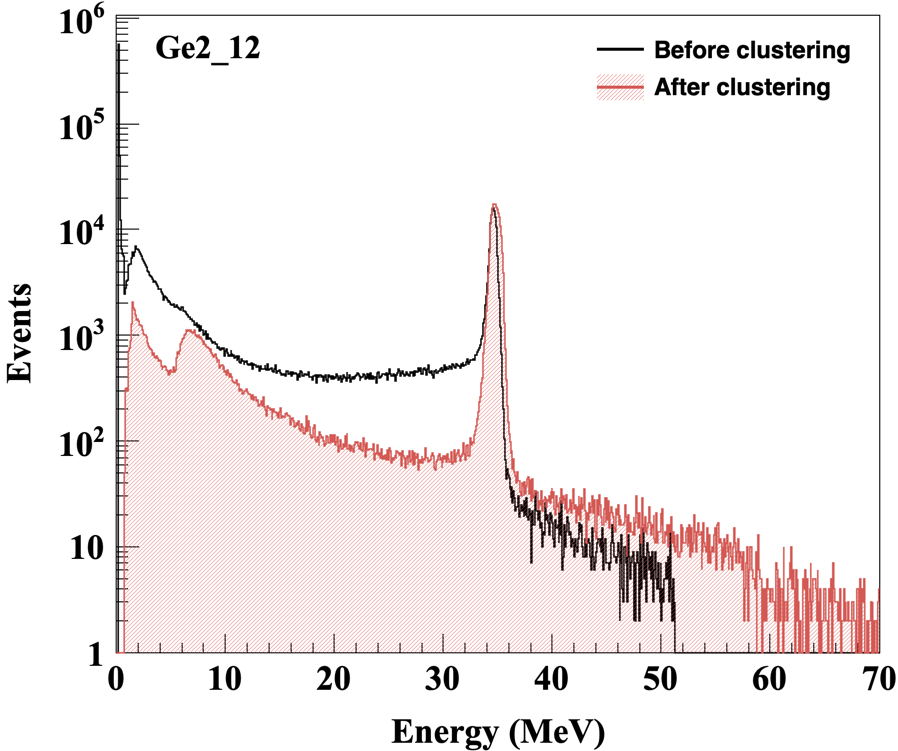
\includegraphics[width=0.45\textwidth]{./clustering.png}
  \caption{Comparison of the energy spectrum on the 12th channel of Ge2, before (black) and after
    (red) clustering.}
  \label{fig:clustering}
\end{figure}
After clustering, part of the hits on the plateau before the elastic peak, which exists in the raw spectrum before clustering, are correctly absorbed into the elastic peak.
% The charasteristics of the background shape also show up with two explicit components: 1) a peak which equals MIP's energy loss in the recoil sensors; 2) a smooth decay with a long tail.
The charasteristic shape of the background spectrum also show up more explicitly.
A correct description of the background shape (see Sec. \ref{sec:recoil_performance})is only possible after clustering.

\subsection{Alignment of the recoil sensors}
\label{sec:alignment}

During installation, the position of the KOALA setup is ajusted accurately based on the
coordinate system of COSY using a laser precisioning system.
However, the relative misalignment between the recoil sensors, which originates from the assembling of the sensor plane , can't be determined in this way.
On the other hand, the exact IP needs to be determined for each experiment run
since it may vary with the running condition of the cluster target.
Thus, alignment based on the experiment data is needed to deduce the accurate recoil angle of the elastic scattering events.

Due to the layout of the recoil sensors, only the alignment along
the beam axis, \textit{i.e.}, Z-axis in the COSY coordinate system, is necessary.
Determination of the alignment parameters is carried out on a sensor basis as follows:
\begin{enumerate}
\item the peak energy of elastic scattering events on each strip is extracted and
  converted to a position along the beam axis based on the kinetics of elastic scattering process;
\item for strips from the same sensor, the difference between the calculated
  position and the position of each strip from the ideal geometry model is filled into the same histogram , as shown in Fig. \ref{fig:alignment};
\item the peak region in the histogram is fitted with a Gaussian to get the
  nominal offset of each sensor against the designed position.
\end{enumerate}
These offsets are the alignment parameters applied in the reconstruction.
Thus, the recoil sensors are aligned so that IP is at the origin of the
laboratory reference frame and the misalignment between the sensors are corrected simultaneously.
\begin{figure}[h!]
  \centering
  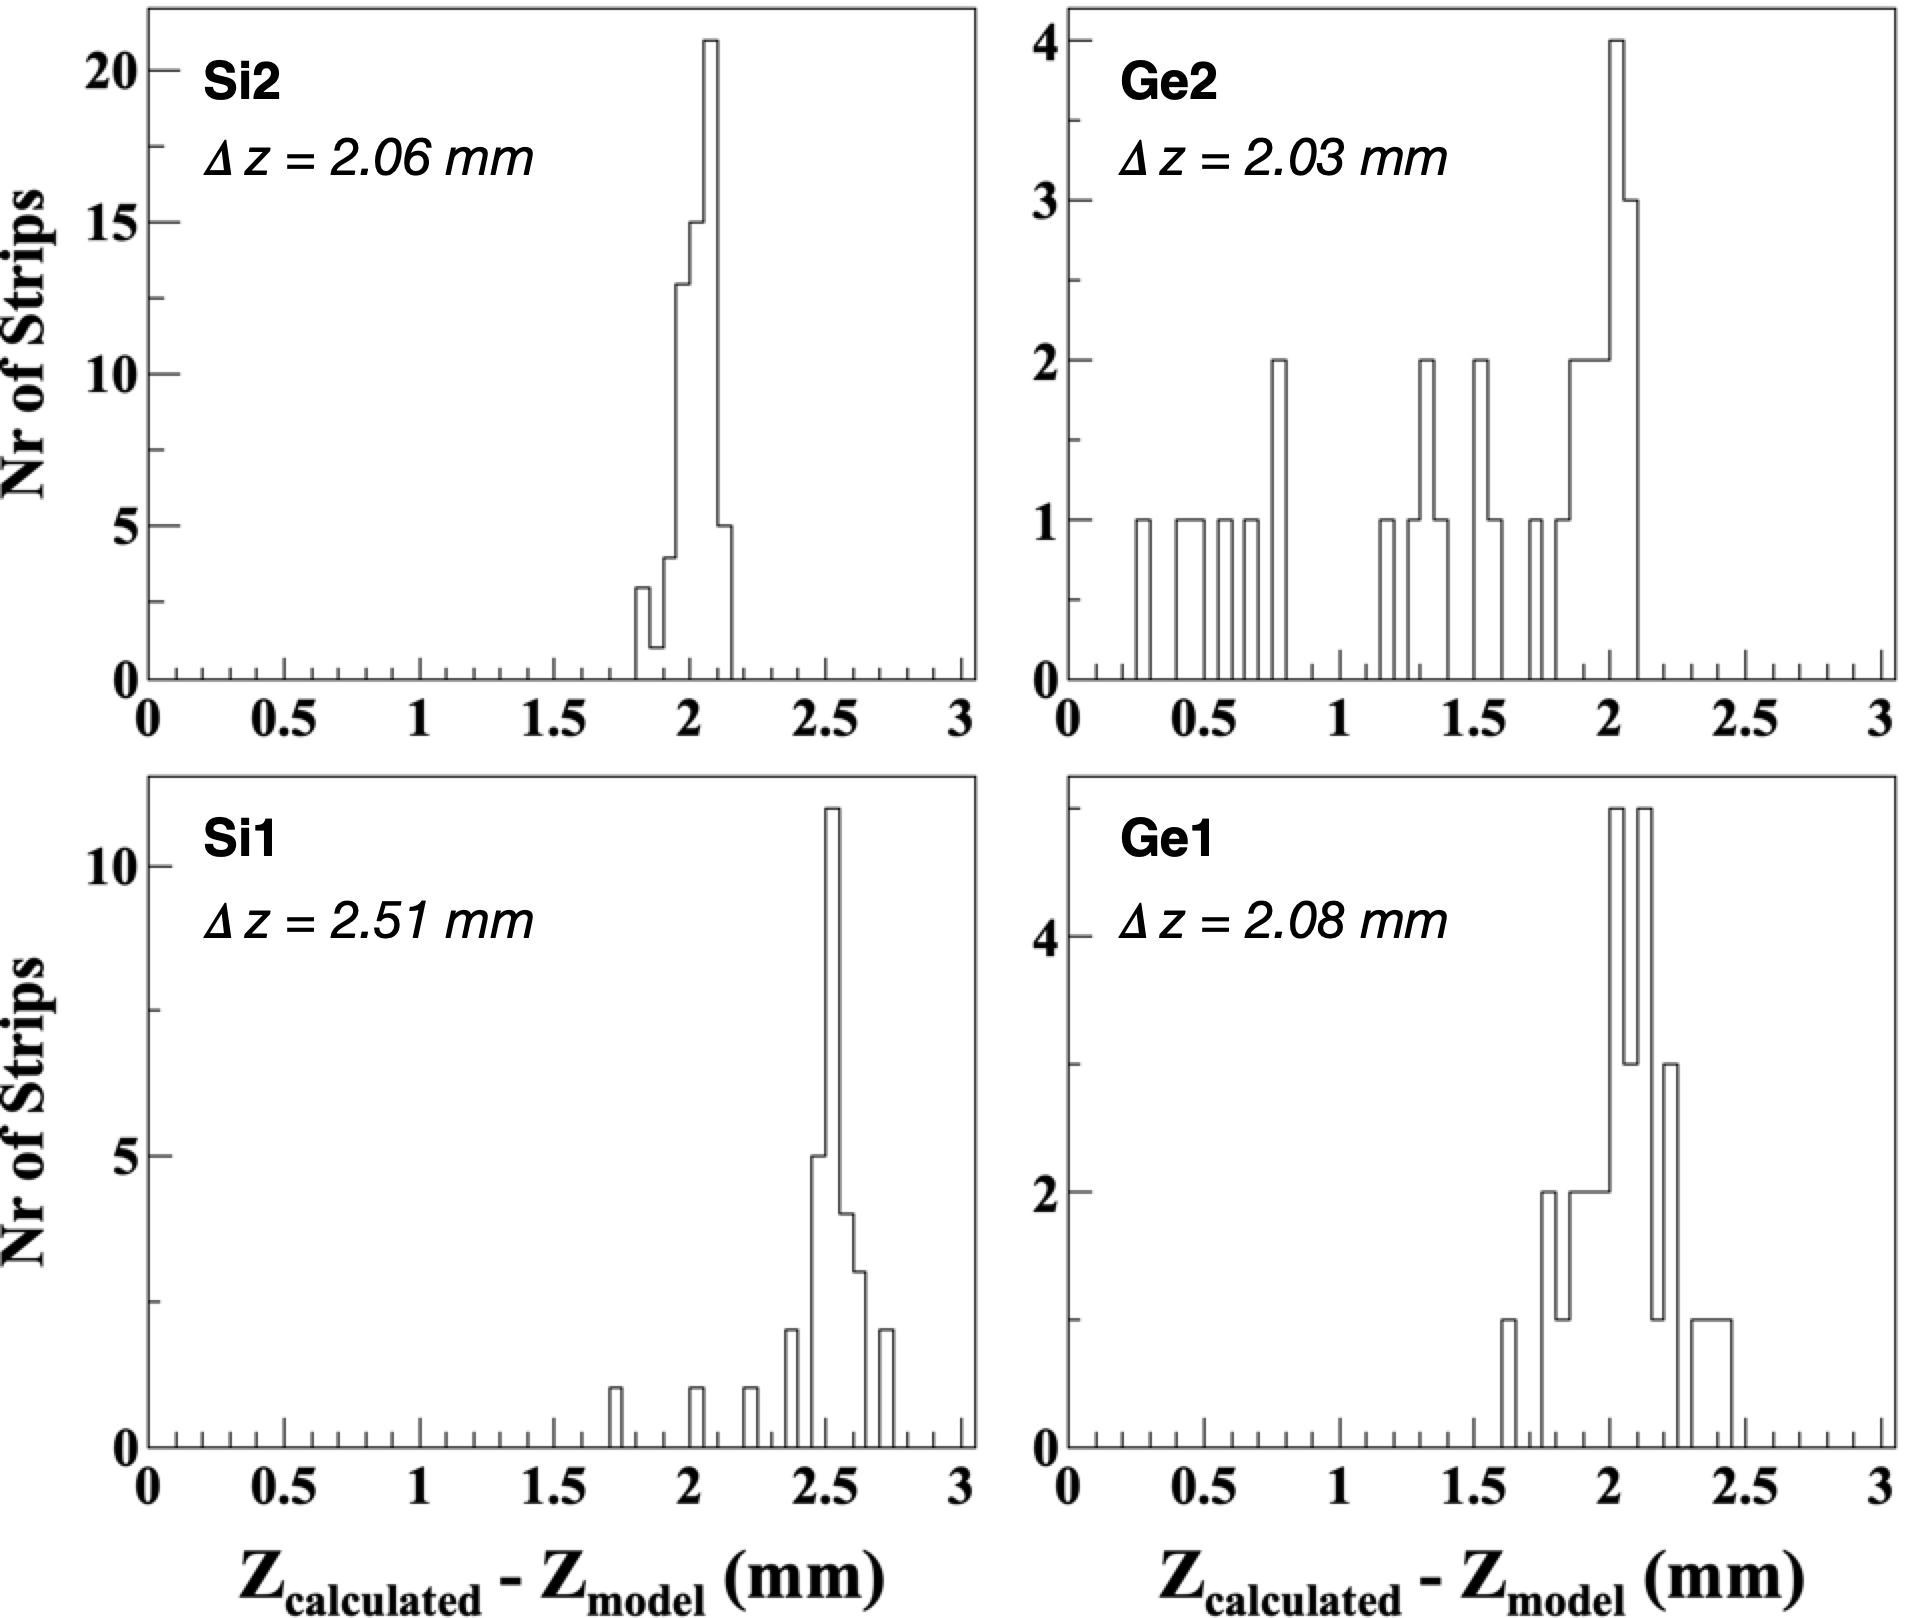
\includegraphics[width=0.45\textwidth]{./alignment.png}
  \caption{Histograms of the difference between the calculated position from the
    elastic peak and the designed position from the geometry model.
    The obtained alignment parameters are
    \SIlist[list-units=single]{2.51;2.06;2.08;2.03}{\mm} for Si1, Si2, Ge1, Ge2 respectively.
    The result is from the data set obtained at $P_{beam} =
    \SI{2.2}{\momentum}$.}
  \label{fig:alignment}
\end{figure}

\section{Beam commissioning and results}
\label{sec:result}

Beam tests were carried out using proton beam at COSY with momentum
\SIlist[list-units=single]{2.2;2.4;2.6;3.0}{\momentum} in August and October, 2019.
% The data analysis procedures of the test beam data are same for all momentums.
In the following, the results from \SI{2.2}{\momentum} are shown as example.

\subsection{Beam conidtion}
\label{sec:beam}
The beam intensity of COSY is about \SI[per-mode=reciprocal]{e10}{\per\second}, with an cycle structure of
\SI{40}{\second} injection time and \SI{300}{\second} storage time, as shown in Fig. \ref{fig:beam}.
To minimize the beam emittance, stochastic beam cooling was applied in these tests.
% The cooling reaches the equibilium state after the beginning $1/3$ of the storage cycle.
\begin{figure}[h]
  \centering
  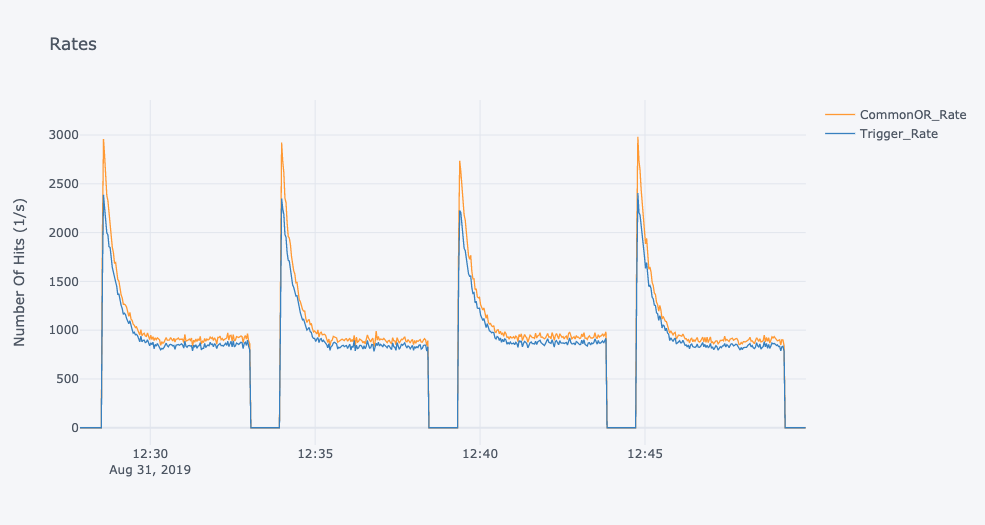
\includegraphics[width=0.45\textwidth]{./daq_efficiency.png}
  \caption{Variation of the total input trigger rates (red) and the ratio between the accepted
    and total input trigger rates (blue) with respect to beam cycling. The ratio
    is a direct measurement of the DAQ efficiency.}
  \label{fig:beam}
\end{figure}
% During injection cycle, the beam has large emittance and not stable.

Only the storage cycle is used for the experiment, which is achieved by two
gates synchronized with the beam cycle.
One gate is used to protect the PMTs of the forward detector during injection
time.
It ramps down the high voltage supply \SI{5}{\second} before the end of the
storage cycle and ramps up the high voltage supply \SI{5}{\second} after the start of the storage cycle.
The other gate has a narrower width and is used to control the DAQ system so that data are not recorded during injection.

The DAQ efficiency in variation with the input trigger rate is also shown in Fig. \ref{fig:beam}.
DAQ was operated under the mask-gate based event synchronization.
A maximum efficiency of \SI{93}{\percent} is reached ,which amounts to \SI{850}{\event\per\second}.
% The efficiency is mainly limited by a wide mask gate in the trigger logic.

\subsection{Performance of the forward detector}
\label{sec:fwd_performance}

% The forward detector shows execellent performance during the beam commisthe
The typical QDC spectra from the two detector modules on the +X aixs are shown as
black curves in Fig. \ref{fig:fwd_performance} (a) and (b).
They are obtained by selecting the events which generate at least one cluster in the recoil detector, \textit{i.e.}, the events which trigger the recoil detector.
The peaks around \num{1200} counts are from the beam particles penetrating
through the scintillators, which have the same energy deposit as MIPs.
The timing resolution (FWHM) of the forward detector is about \SI{400}{ps}, which is determined from the spread of the timing difference between the two module as show in Fig. \ref{fig:fwd_performance} (c).

% A further study is carried out with the sample of elastic scattering events (the selection of the elastic scattering events are described in Sec. \ref{sec:elastic_extraction}).
% The peaks lie above a continuum background, in which no distinctive thresholds can be recognized to separate the noise pedestal and the peak.
A further study is carried out using the tag-and-probe method with a controlled
sample of elastic scattering events.
The response of one module is probed by using the other module to tag the sample
(the procudures of selecting the elastic scattering events are described in the
next section).
The results are shown as the red shaded curves in Fig. \ref{fig:fwd_performance}.
The lower limit of the spread of elastic peaks are clearly seen around \num{1000}.
In the following analysis, this value are used as the threshold to determine the firing of the forward detector.
Corresponding SNRs are about \num{40} for both detector modules.
\begin{figure}[htb!]
  \centering
  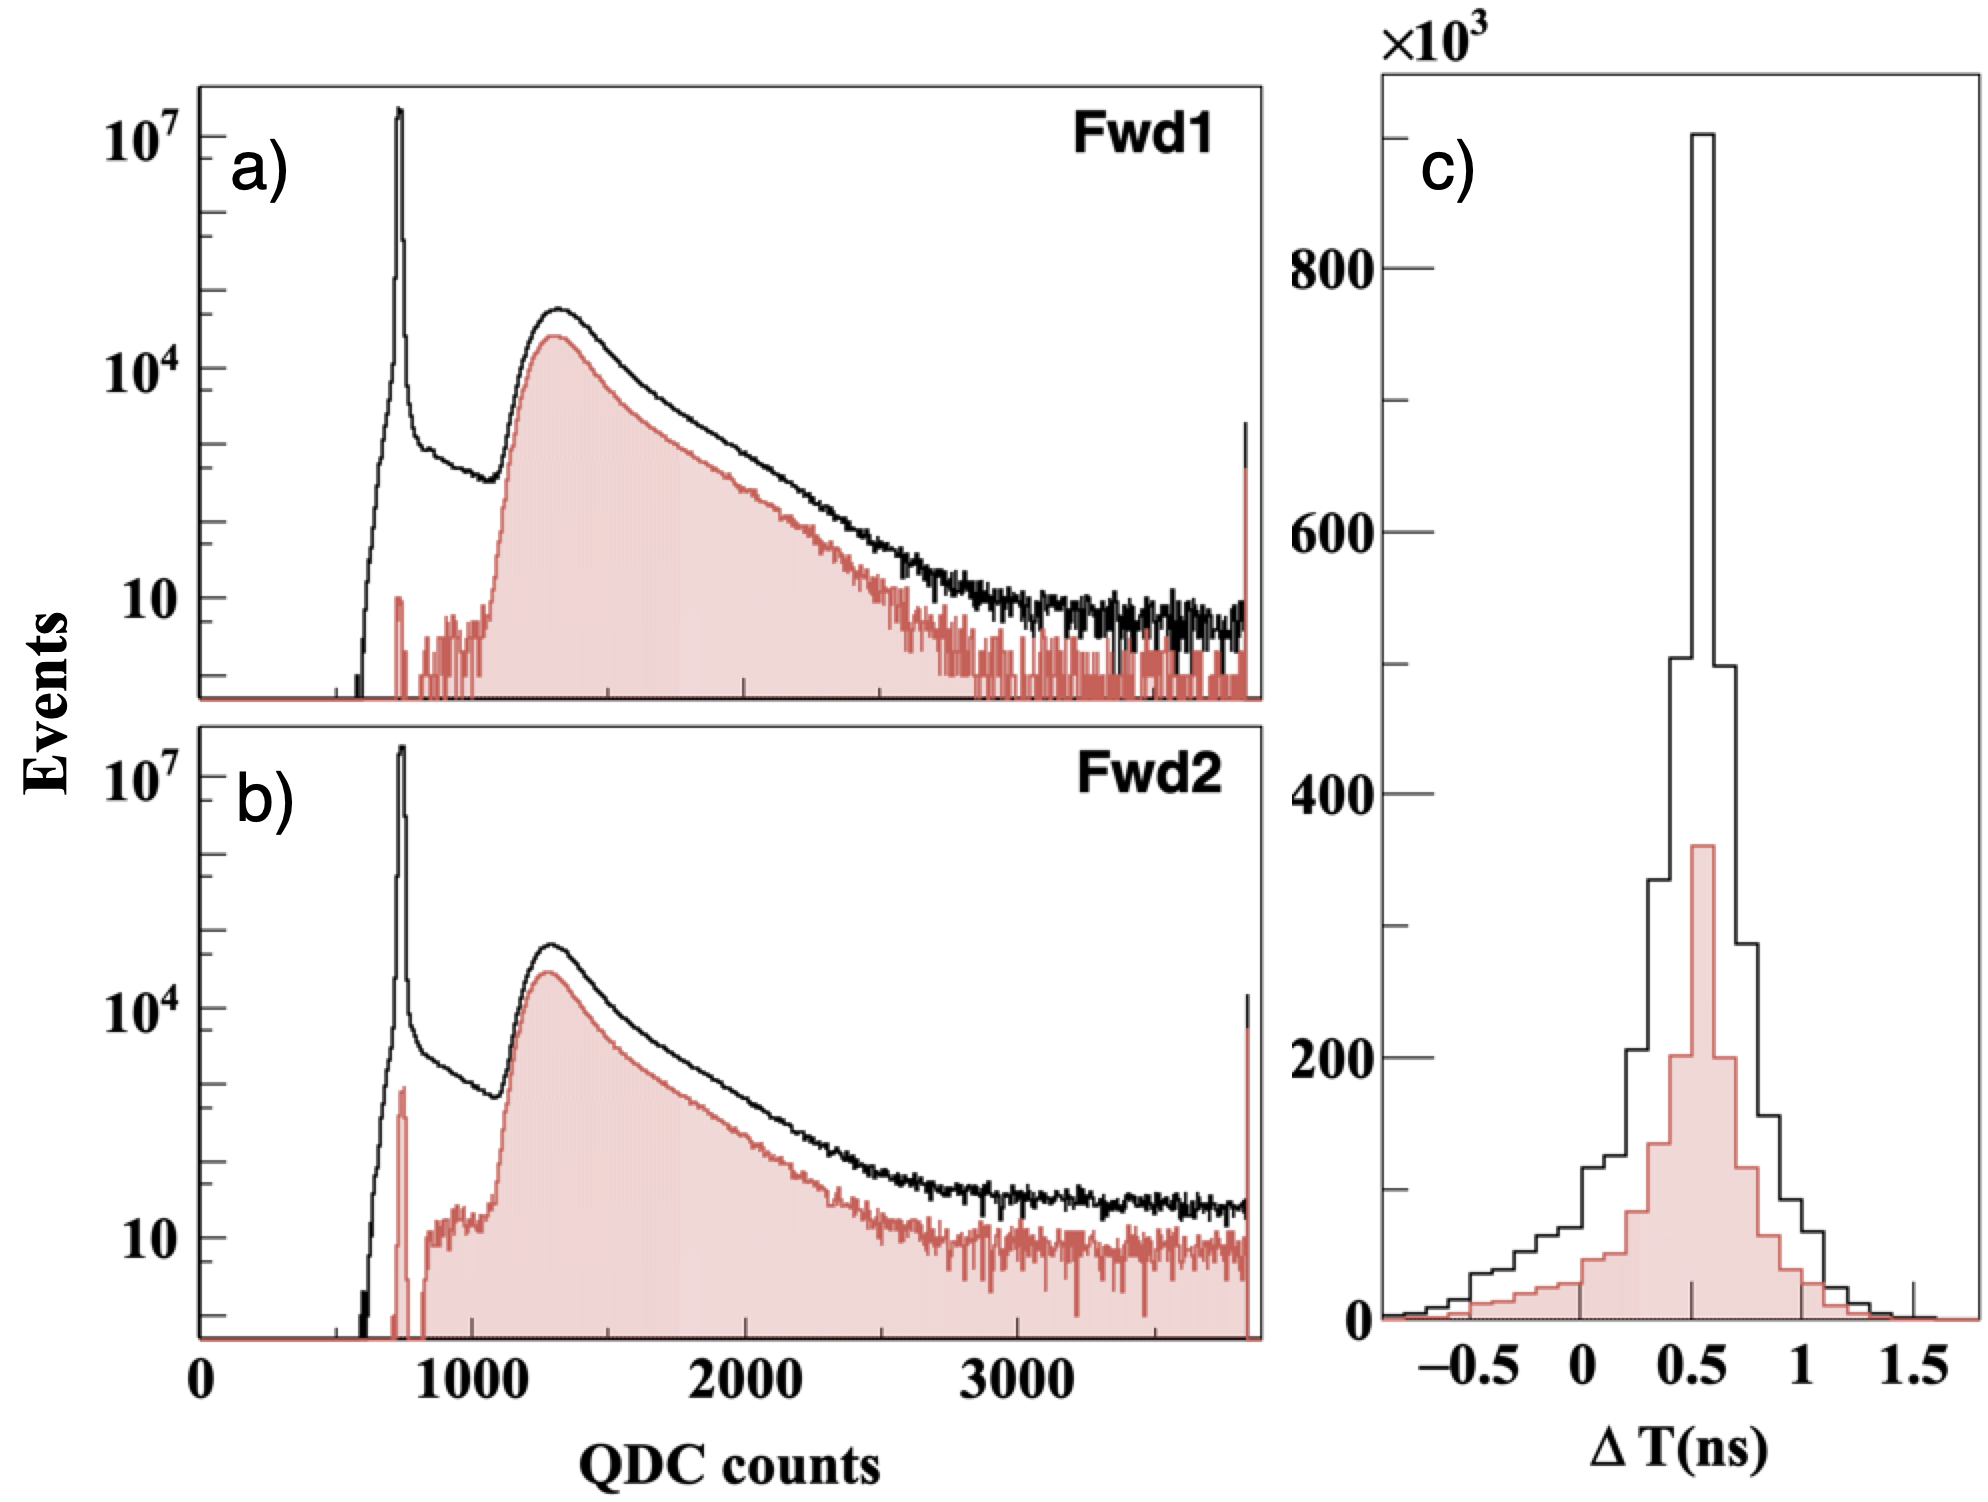
\includegraphics[width=0.45\textwidth]{./fwd_performance_elastic.png}
  \caption{Response of the forward detector: a) the QDC spectrum of the first forward detector module on +X axis;
    b) the QDC spectrum of the second forward detector module on +X axis; c) Time difference between these two modules.
    The black curve are from the events which are triggered by the recoil
    detector.
    The red shaded curve are from the elastic scattering event sample.
  }
  \label{fig:fwd_performance}
\end{figure}

The detection efficiencies of the forward modules are also determined with the
tag-and-probe method, which are about \SI{99.9978}{\percent} and \SI{99.9560}{\percent} respectively.
The scattering effect in the first layer reduces the detection efficiency slightly in the second layer.
% Due to the high efficiency, the joint firing of them are required to select a
% valid hit in the forward detector and the hit time is the average of two modules.
The joint firing of both modules are required to have a valid hit in the
forward detector and the hit time is the average of two modules.

% \subsection{Extraction of elastic scattering peak at large recoil angle}
\subsection{Performance of the recoil detector}
\label{sec:recoil_performance}
The reconstructed energy spectra of the recoil detector show a clear pattern
of elastic scattering in the distribution of the deposited energy versus the
position along the beam axis as shown in Fig. \ref{fig:e_map}.
The elastic peaks lie upon a wide spread of background, which exists over the whole energy range.
The peaks are well seperated from the low-energy background at large recoil angles, while they are hard to distinguish at small recoil angles.
Three components are recognized in the background spectrum:
1) a fast-decreasing exponential component, which has very high yield at low energy;
2) a slow-decreasing exponential component, which extends to very high energy;
3) a MIP component, which can be described well by the Landau distribution and has a most probable energy deposit of \SI{0.37}{\MeV} in Si1 and Si2, \SI{2.2}{\MeV} in Ge1 and \SI{7.0}{\MeV} in Ge2.
The MIP events are mainly generated by the pions from inelastic interactions.
\begin{figure}[htb!]
  \centering
  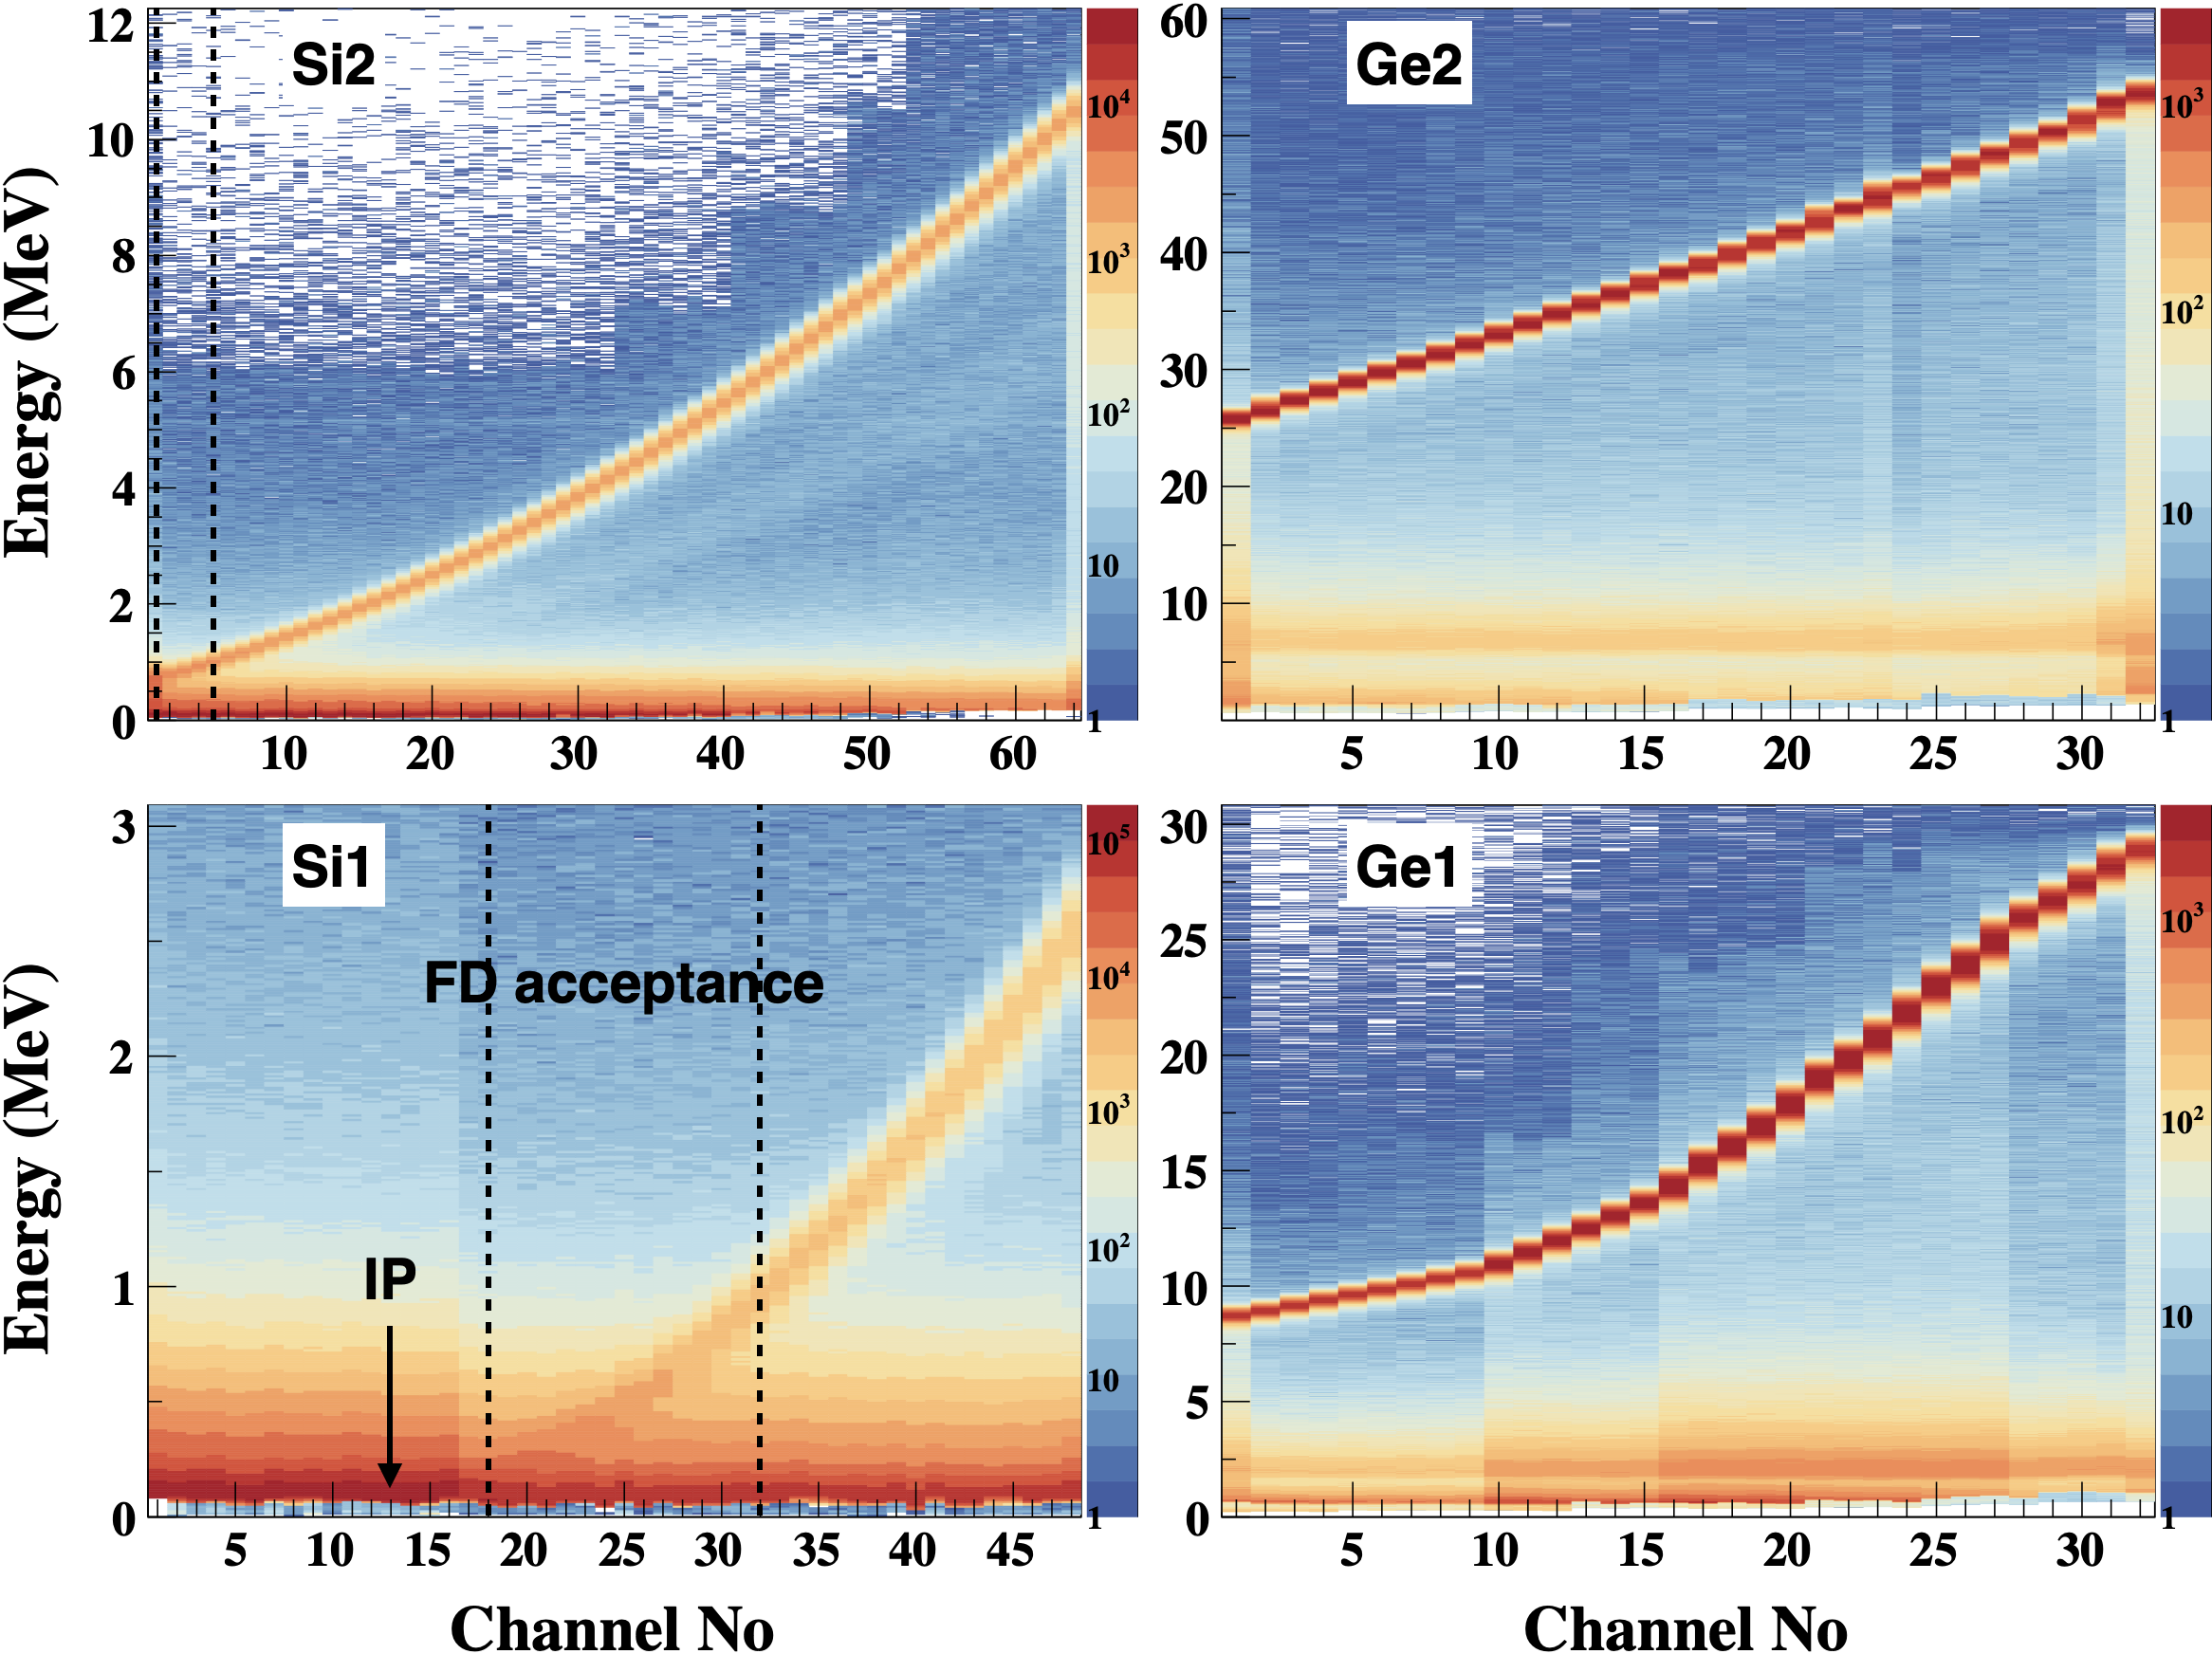
\includegraphics[width=0.48\textwidth]{./e_map.png}
  \caption{Energy spectra (after clustering) of all channels of the four recoil
    sensors obtained at \SI{2.2}{\momentum}.
    Lower channel number indicates smaller recoil angle.
    IP indicates the channel which is in alignment with
    the beam-target center.
    The group of channels which are fully covered by the forward detector are
    also indicated by the dashed lines on Si1 and Si2.
  }
  \label{fig:e_map}
\end{figure}

The response of each strip to the elastic scattering events from IP is described
very well by the Crystal-Ball function\cite{crystal_ball}, which is composed of a Gaussian core and a power-law tail on each side of the core.
For the strips at large recoil angle, an accurate estimate of the parameters of
the backgroud components is possible by fitting the sidebands around the elastic peak.
Extended binned Maximum-Likelihood fit over the full energy range, including both the background and the
elastic peak, is then carried out to extract the parameters of the response function and the event rate under the peak.
An example of the combined fit is shown in Fig. \ref{fig:e_fit}.
% The sum of multiple Cystal-Ball functions, which share the same shape parameters and
% different Gaussian peaks, are used to desribe the response of the readout channel with multi-strips. 
% The standard one-sided Crystal-Ball distribution is expanded to double sides, which is composed of a Gaussian core and two
% power-law tails at low-end and high-end of the core.
% The extracted width of the response function core varies with the peak energy and the
% equivalent Fano factor is about 185 larger than the one obtained using $\alpha$
% source, which is about 17 in terms of FWHM.
The instrinsic resolution of the recoil sensor determined from the $\alpha$ source
calibration ($\sim$\SI{20}{\keV} in terms of FWHM at \SI{5}{\MeV}) is much smaller than the extracted width of the elastic peak from the beam commissioning data ($\sim$\SI{330}{\keV} at the same energy as the $\alpha$ source).
Thus, the energy resolution in the experiment is mainly dominated by the finite angular converage of the strip and the thickness of the cluster target along beam-axis.
\begin{figure}[h!]
  \centering
  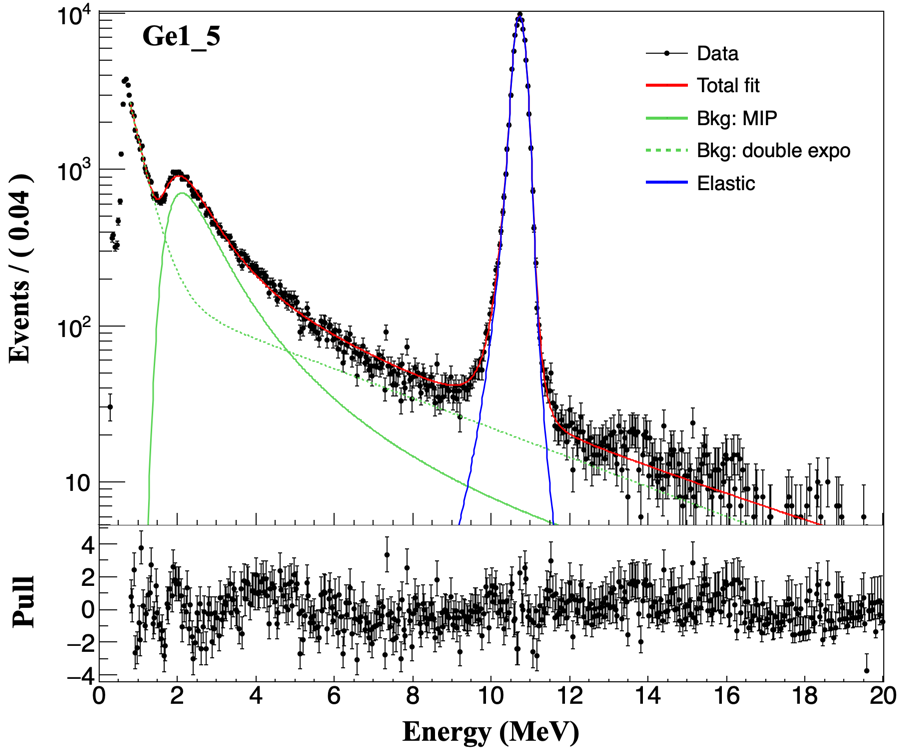
\includegraphics[width=0.45\textwidth]{./e_fit.png}
  \caption{Extraction of the elastic peak of Ge1\_6 using the extended binned
    Maximum-Likelihood fit. Three components are used in the background model
    and the fit is carried out over the full energy range. The pull of each bin
    is shown in the bottom subplot.}
  \label{fig:e_fit}
\end{figure}

The accuracy of the combined fit deteriates at small recoil angles, when the elastic peak is close to the MIP peak and both peaks are embeded among the large
low-energy background ($\lesssim$ \SI{1}{\MeV}).
In this case, it's hard to estimate the parameters of the background components
through the sideband fit, and there is a large error in determining the fraction of
each component.
A pre-selection of the elastic scattering events is needed to get a cleaner spectrum.
For the strips which are covered by the forward detector, the correlation
between the recoil proton and the scattering beam particle is utilized for this selection.

% The fitting model is composed as follows,
% \begin{equation}
% \begin{aligned}
% \mathcal{P}(x) &= N_{1}\lambda_1e^{-\lambda_{1}x}+N_{2}\lambda_2e^{-\lambda_{2}x}\\
% &+N_{3}\mathcal{L}(x;\mu_{mip},\sigma_{mip})\ast\mathcal{N}(x;\sigma_{gaus})\\
% &+N_{4}\sum_{i=1}^{n_{strips}}{c_{i}f(x;\mu_{i},\sigma_{cb},\alpha_1,n_1,\alpha_2,n_2)}
% \mathcal{P}(x) &= N_{1} \cdot exp(x;\lambda_{1}) + N_{2} \cdot exp(x;\lambda_{2})\\
% &+ N_{3}\cdot L(x;\mu_{mip},\sigma_{mip}, \sigma_{res})\\
% &+ N_{4}\cdot \sum_{i=1}^{n_{strips}}{c_{i}f_{cb}(x;\mu_{i},\sigma_{cb},\alpha_1,n_1,\alpha_2,n_2)}
% \end{aligned}
% \end{equation}
% where the first two items are the exponential components, the third item is the
% normalized landau distribution convoluted with the Gaussian response function
% and the fourth item is the response function of the recoil detector to the
% elastic scattering events from the target.
% $N_i (i=1,2,3,4)$ is the event counts for each component of the model.
% The double-sided crystal ball function is composed of a Gaussian core and two
% power-law tails as follows,
% \begin{multline}
%   f(x;\mu,\sigma,\alpha_1,n_1,\alpha_2,n_2) = \\
%   N\cdot
%   \begin{cases}
%     \exp(-\frac{(x-\mu)^2}{2\sigma^2}), &\text{for } \alpha_1 < \frac{(x-\mu)}{\sigma} < \alpha_2\\
%     A_1(B_1-\frac{x-\mu}{\sigma})^{-n_1}, &\text{for } \frac{(x-\mu)}{\sigma} \leqslant \alpha_1\\
% 	    A_2(B_2+\frac{x-\mu}{\sigma})^{-n_2}, &\text{for } \frac{(x-\mu)}{\sigma} \geqslant \alpha_2
%   \end{cases} 
% \end{multline}
% where
% \begin{align}
%   A_i &= (\frac{n_i}{\abs{\alpha_i}})^{n_i}\cdot\exp(-\frac{\alpha_i^2}{2}) &,(i=1,2)\\
%   B_i &= \frac{n_i}{\abs{\alpha_i}} - \abs{\alpha_i} &,(i=1,2)
% \end{align}

\subsection{Event selection with the TOF-E relation}
\label{sec:tofe_selection}

Most background events are already supressed by requiring that the forward detector has a valid
hit from the beam particle.
The more accurate selection of elastic scattering events is achieved by using the TOF-E relation.
The time-of-flight (TOF) of the recoil proton and its kinetic energy (E)
have a fixed relation $TOF = l\sqrt{m_p/2E}$, where $l$ is the distance of
the recoil detector to IP and $m_p$ is the proton mass.
Due to the small variation of the flight time of the scattering beam particle,
TOF of the recoil proton can be approximated by the difference between the hit time of the recoil detector and the forward detector.

% Elastic selection based on TOF-E
% The typical TOF-E spectrum from a single strip is shown in the inner subplot of Fig. \ref{fig:tof-e}.
Two bands of events, which split from the elastic peak, are observed in the raw TOF-E spectrum on each strip, as shown in the inner subplot of Fig. \ref{fig:tof-e}.
Both bands are generated by the elastically-recoiled protons, with: 1) band A from
the the interaction of the beam particle with the residual gas in the beam pipe; 2)
band B from the events in which the recoil protons hit the edge of the strip and
deposit partial energy in the sensor.
\begin{figure}[h!]
  \centering
  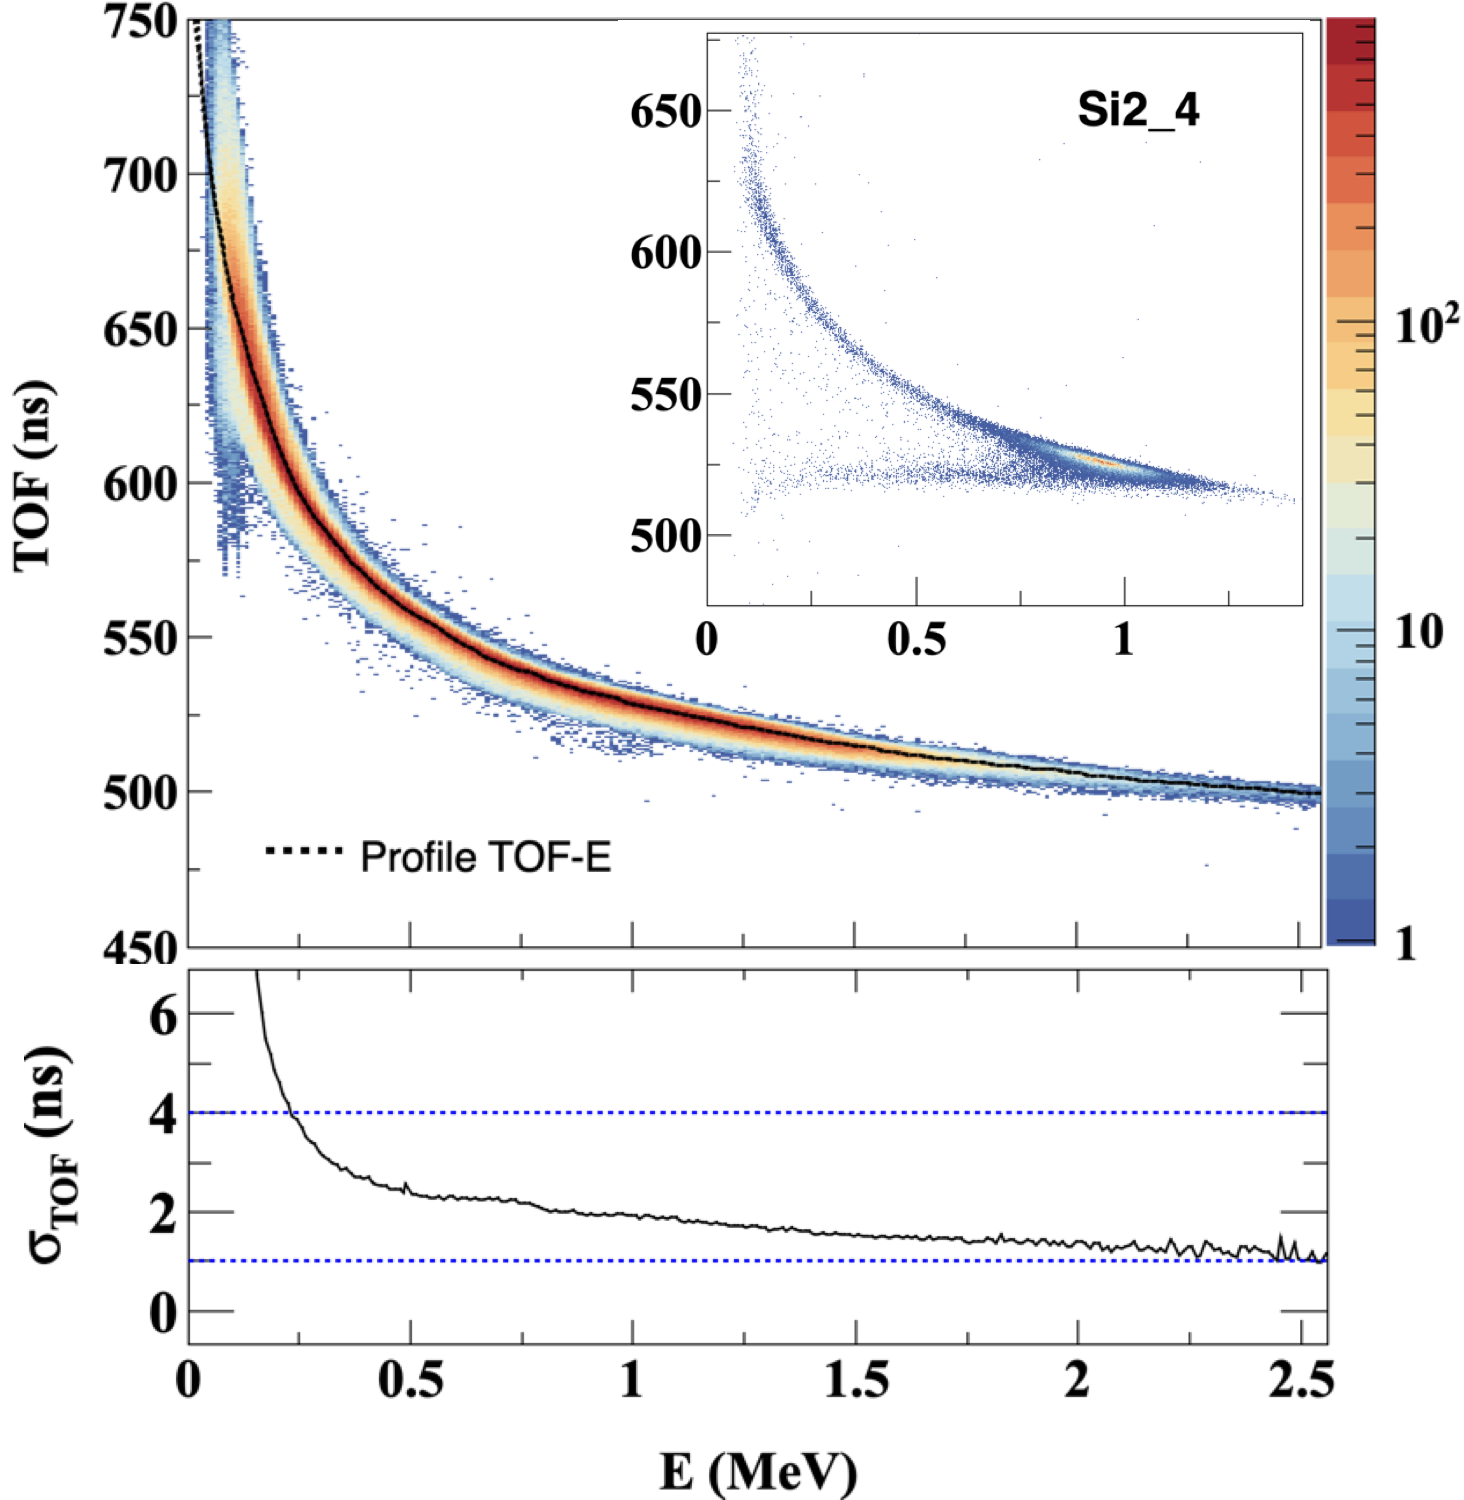
\includegraphics[width=0.45\textwidth]{./tofe_tsigma.png}
  % 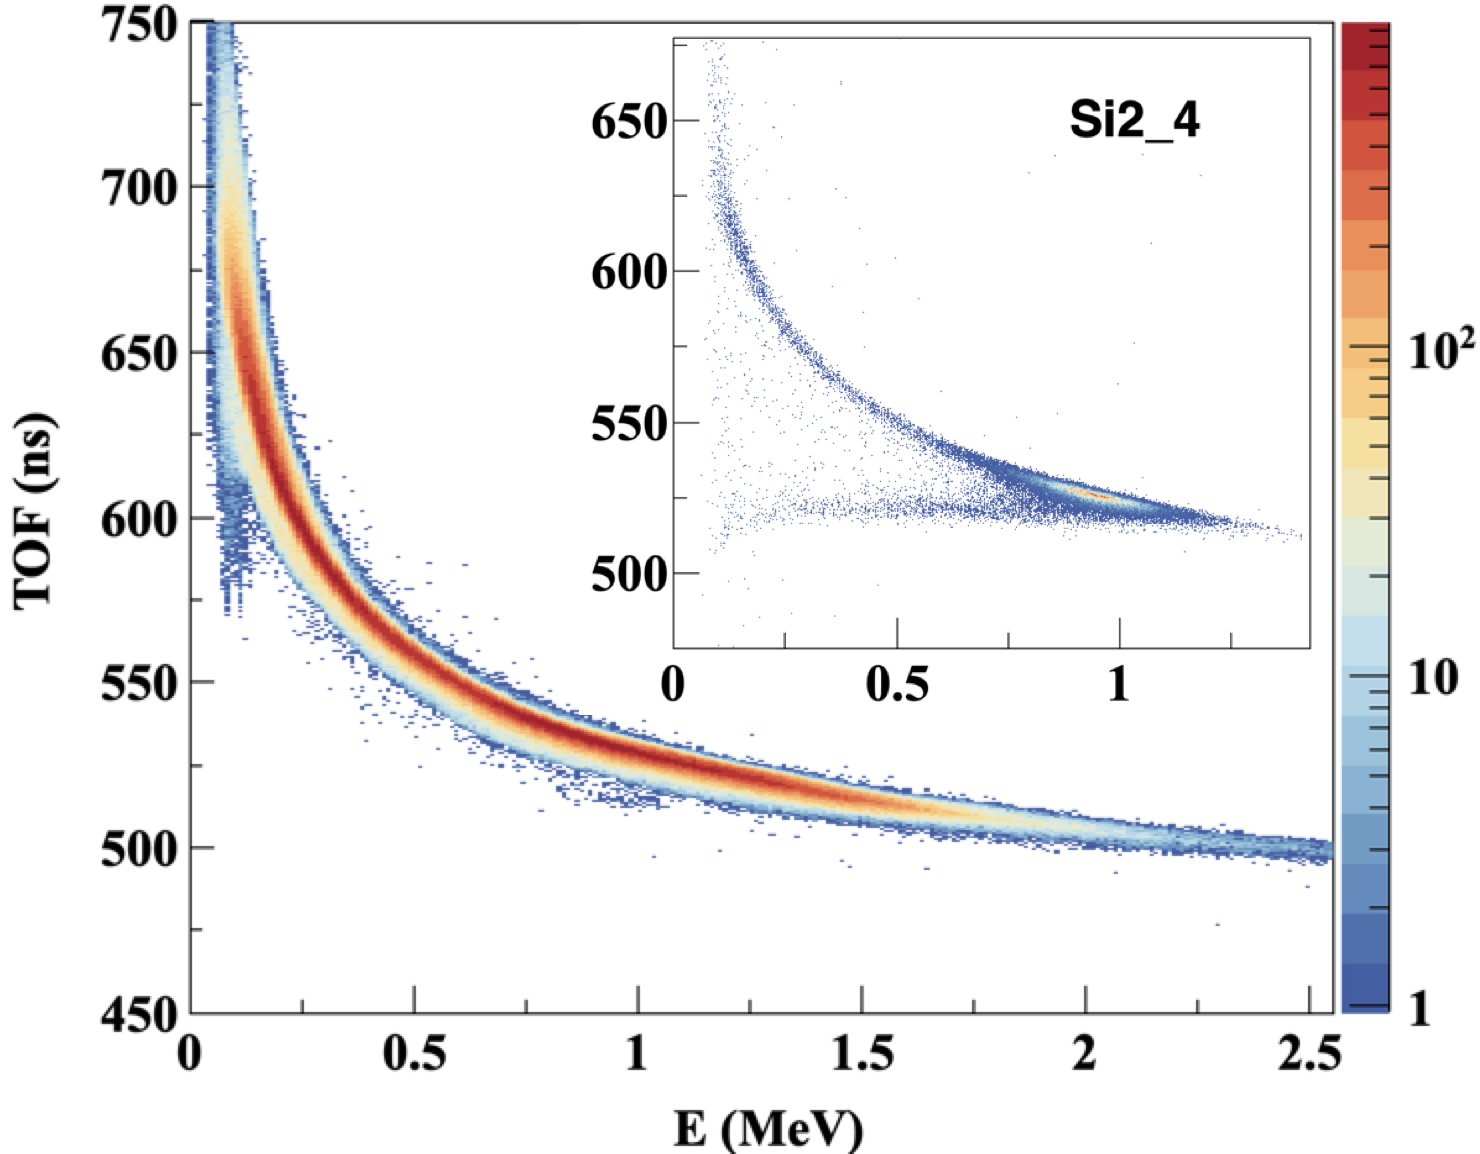
\includegraphics[width=0.4\textwidth]{./tofe_cut.png}
  \caption{
    The overall TOF-E spectrum of selected elastic scattering events at
    \SI{2.2}{\momentum} and its associated TOF-E curve obtained from profiling
    along E-axis.
    Typical raw TOF-E spectrum on a single strip is shown in the inner subplot.}
  \label{fig:tof-e}
\end{figure}
The events of the elastic peak and band A are cut out roughly and filled into an
overall TOF-E spectrum of elastic scattering events from all strips.
This spectrum is profiled every \SI{10}{\keV} step along the E-axis,  and a
smooth, data-deduced TOF-E curve is obtained as show in the main plot of Fig. \ref{fig:tof-e}.
The standard deviation of TOF ($\sigma_{TOF}$) at each step is also extracted and shown in the bottom plot of Fig. \ref{fig:tof-e}.
$\sigma_{TOF}$ reaches a limit value of $\sim$\SI{1}{\ns} at very large energy,
which can be considered as the intrinsic timing resolution of the recoil
detector since the forward detector has much smaller resolution (see Sec. \ref{sec:fwd_performance}).
At $E < \SI{250}{\keV}$, $\sigma_{TOF}$ is dominated by the large derivative
of the TOF-E relation and deteriates rapidly.
% This selection effectively filter out all the full elastic events as show in the
% main plot of Fig. \ref{fig:tof-e}.
% \textit{i.e.} elastic events in which the recoil proton deposit all its energy in the recoil sensor and the scattered proton penetrating through the forward detector. 
% The TOF-E spectrum The selected events from all of this selection is shown in Fig. \ref{fig:tof-e}.
% with the two side plots showing the variation of the
% standard deviation ($\sigma_{TOF}$ and $\sigma_{E}$) of the profile along the E-axis and TOF-axis respectively.
% The deteoriation of the resolution near the edge of the spectrum is mainly
% contributed by the extremely large or small derivative of the TOF-E curve at
% these energy values.
% The modest value of $\sigma_{TOF}$ and $\sigma_{E}$ is about
% \SI{2.5}{\nano\second} and \SI{25}{\keV} respectively.

% combined fit using coulomb background and coverage of the fwd acceptance
The TOF-E curve is combined with a $[-5\sigma_{TOF}, 5\sigma_{TOF}]$ window to select the elastic scattering events on each strip.
A clean energy spectrum is obtained after the selection and the elastic peak shows up clearly.
Results from three strips at different recoil angles are shown in Fig. \ref{fig:cut}.
For strips which are fully covered by the forward detector, the spectrum of the
surpressed background events has a smooth transition over the elastic peak range
as shown in Fig. \ref{fig:cut} (b).
This indicates a high efficiency of the selection condition.
With increasing recoil angle, the forward detector gradually loses the coverage
of the recoil strip and a small elastic peak appears in the background spectrum
as shown in Fig. \ref{fig:cut} (c).
On the other hand, with decreasing recoil angle, the target thickness can't be
ignored and the forward detector starts to lose the coverage of the full target profile due
to the lower limit of the acceptance as shown in Fig. \ref{fig:cut} (a).

The remaining background in the selected events comes from the elastic scattering off the residual gas.
% The spectrum of the selected elastic events has a contribution from the residual
% gas interaction.
The shape of this background is well described by the Coulomb elastic scattering cross
section, due to the uniform distribution of the residual gas and the rapid decrease of the elastic scattering cross section beyond the Coulomb region.
Extended unbinned Maximum-Likelihood fit with a summed model of the Coulomb elastic scattering formula and the Crystal-Ball
function is used to extract the parameters of the response function and the yield of elastic events from the target body. 
The fit results for the three example strips are also shown in Fig. \ref{fig:cut}.
It's found that the fit quality deteriates when the full shape of the target profile is not available in the selected spectrum.
This limits the lower range of $|t|$ measurement to $\sim$\SI{0.001}{\tmom} at $P_{beam}=\SI{2.2}{\momentum}$.
\begin{figure}[h!]
  \centering
  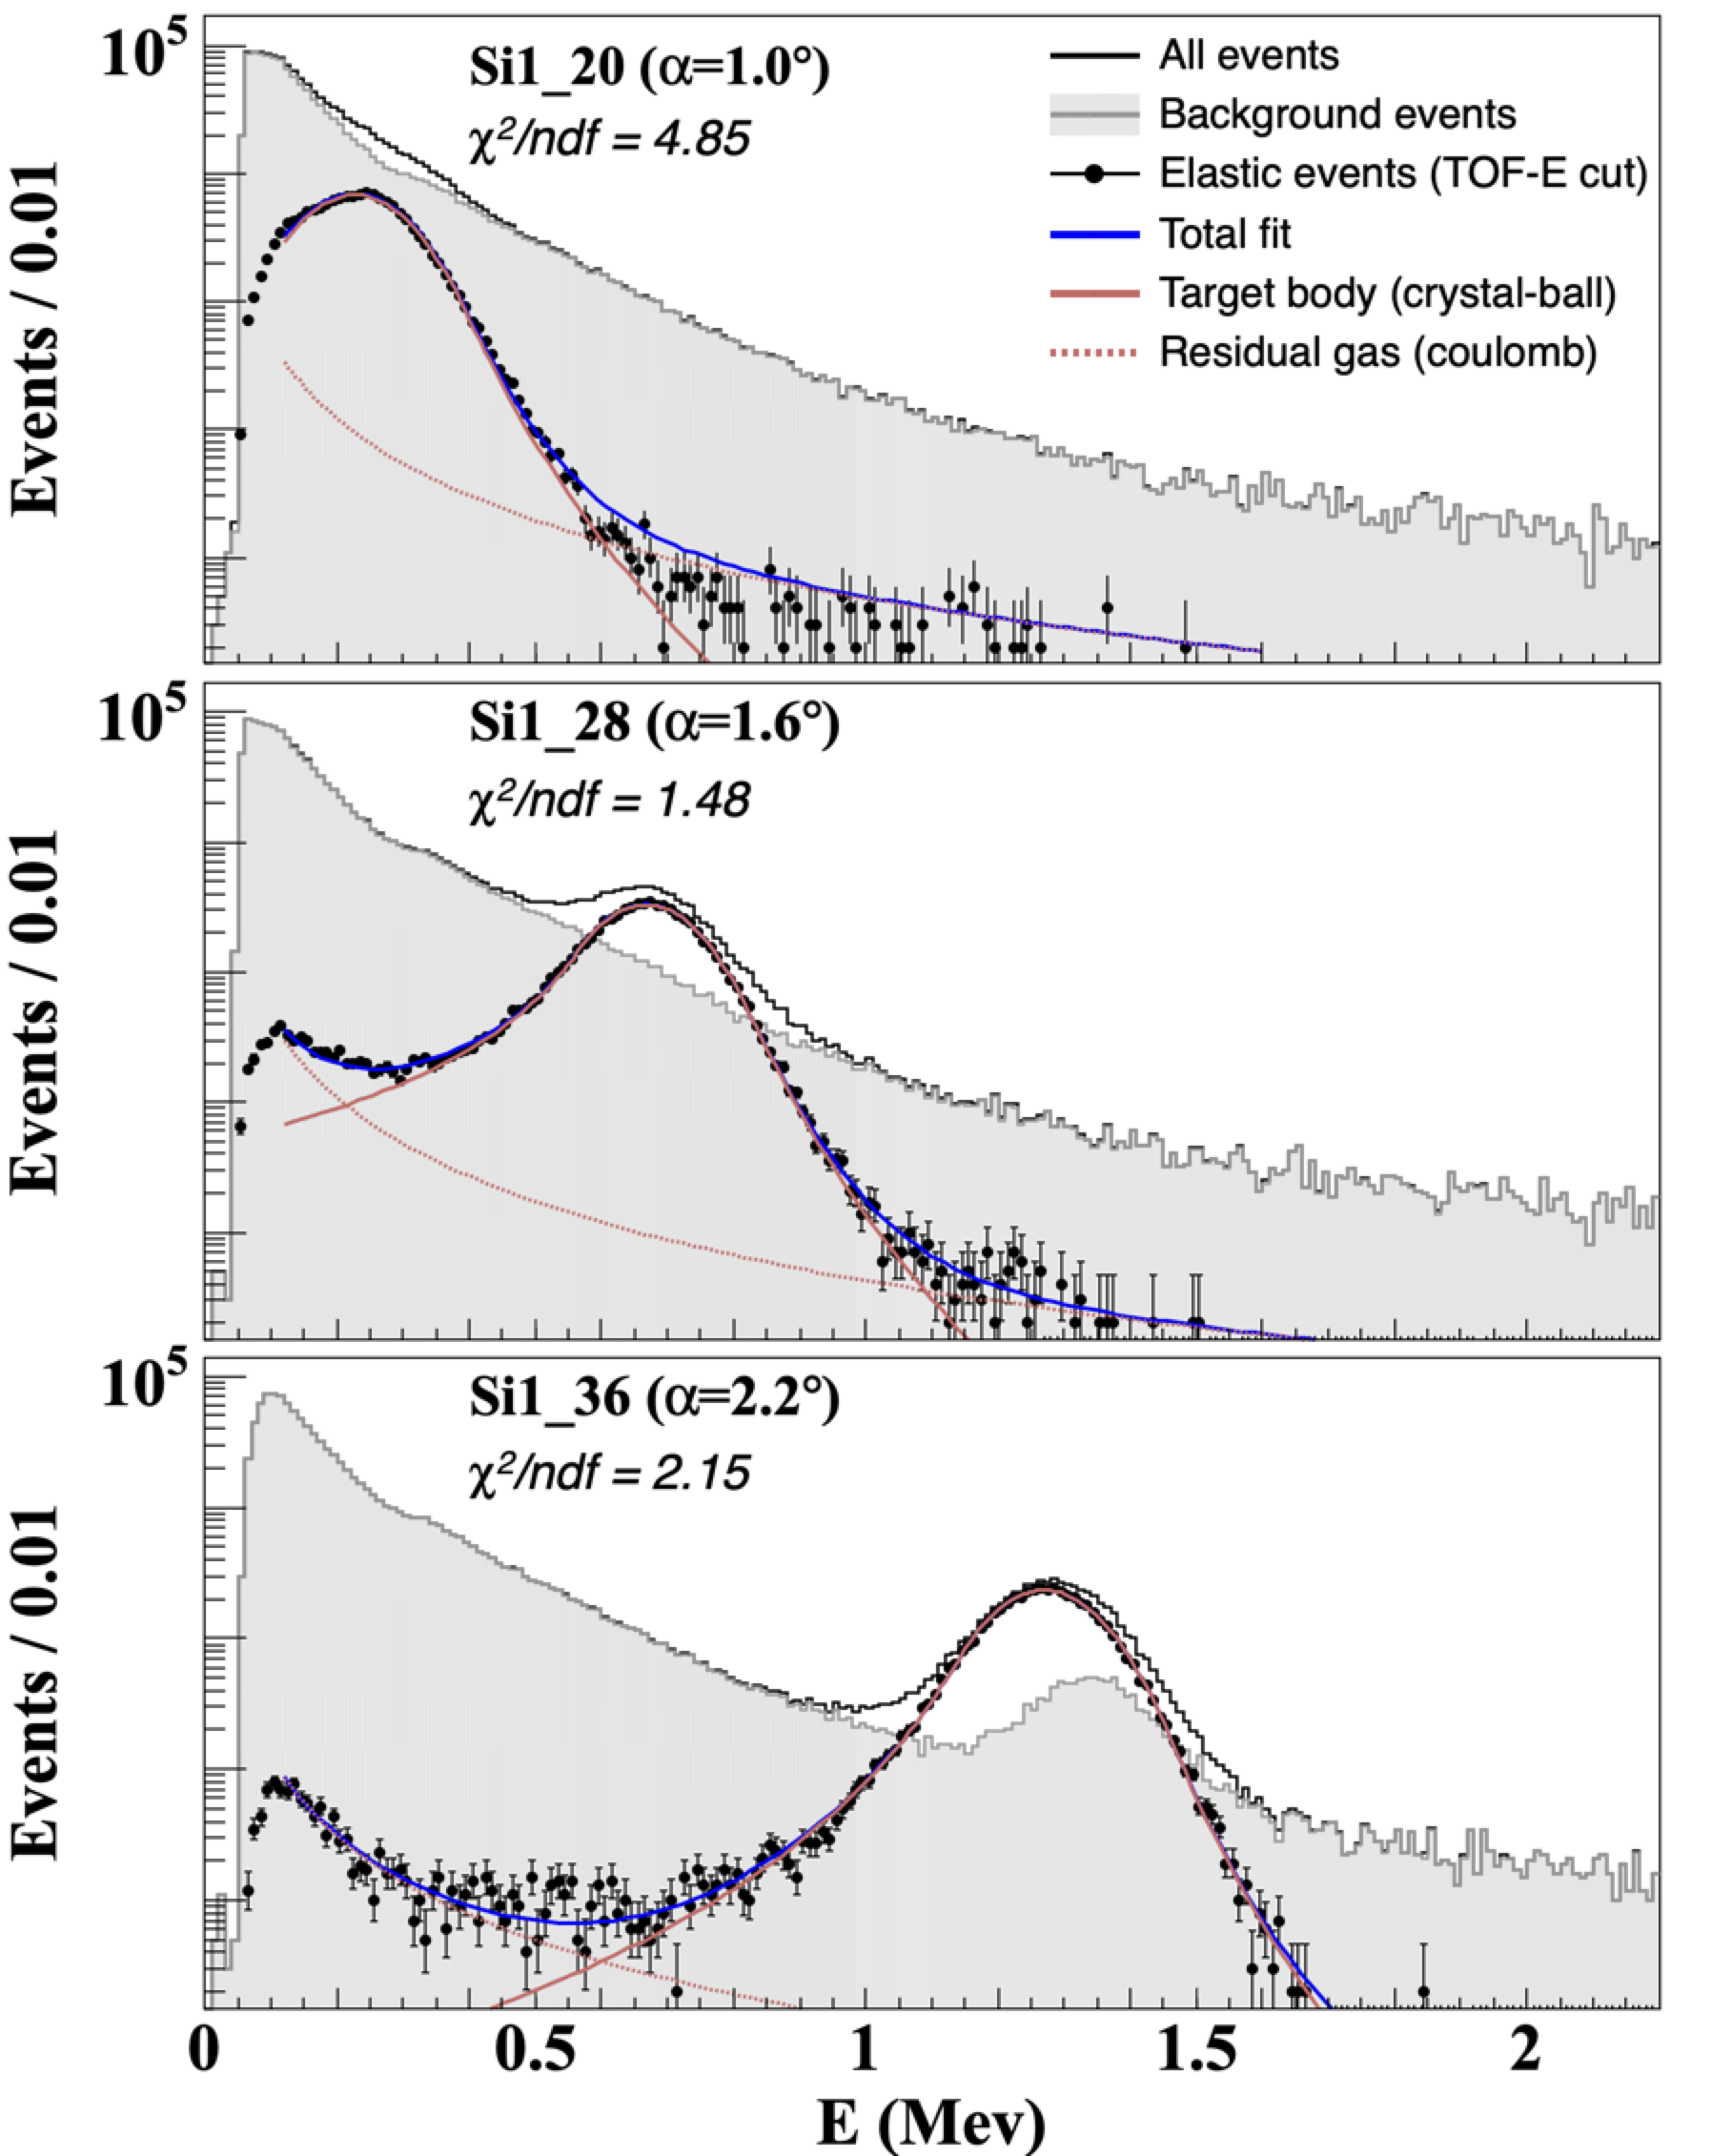
\includegraphics[width=0.45\textwidth]{./tofe_cut_comparison.png}
  \caption{The energy spectra of TOF-E selected events (black dots) from strips at
    three recoil angles. The black lines are from all events and the grey areas
    are from the supressed background events.}
  \label{fig:cut}
\end{figure}


\subsection{Minimum measurable $|t|$}
\label{sec:minimum_t}
The spectra of the supressed background events on the strips which are fully covered by the
forward detector can be used as the template model to describe the background
shape on strips at smaller recoil angles.
Thus, the lower range of |t| measurement is extended below the limit of the TOF-E selection method.
The scaling parameter of the background model is first estimated with the upper
sideband of the energy spectrum, and a combined fit with the summed
model of the Crystal-Ball function and the background template is then carried
out over the fully energy range to extract the elastic peak spectrum.

% A limit is observed around \SI{350}{\keV}, which corresponds to $|t| \approx  \SI{0.0007}{\tmom}$.
The limit of the method is reflected in the extracted elastic peak energy on each strip as shown in
Fig. \ref{fig:measured_vs_calculated}.
For the strips where the full elastic peak spectrum is extracted and described accurately
by the Crystal-Ball function, the relative difference between the measured and
the calculated recoil energy based on kinematic relations is within \SI{\pm 1}{\percent}.
The discrepancy enlarges rapidly at $\alpha < \SI{1.2}{\degree}$ when part of
the target profile is not recorded by the recoil strips due to the trigger threshold.
Both the extracted parameters of the response function and the event rate have large uncertainties in this case.
The observed limit corresponds to the minimum measurable $|t|$ of $\sim$\SI{0.0007}{\tmom}.
\begin{figure}[h!]
  \centering
  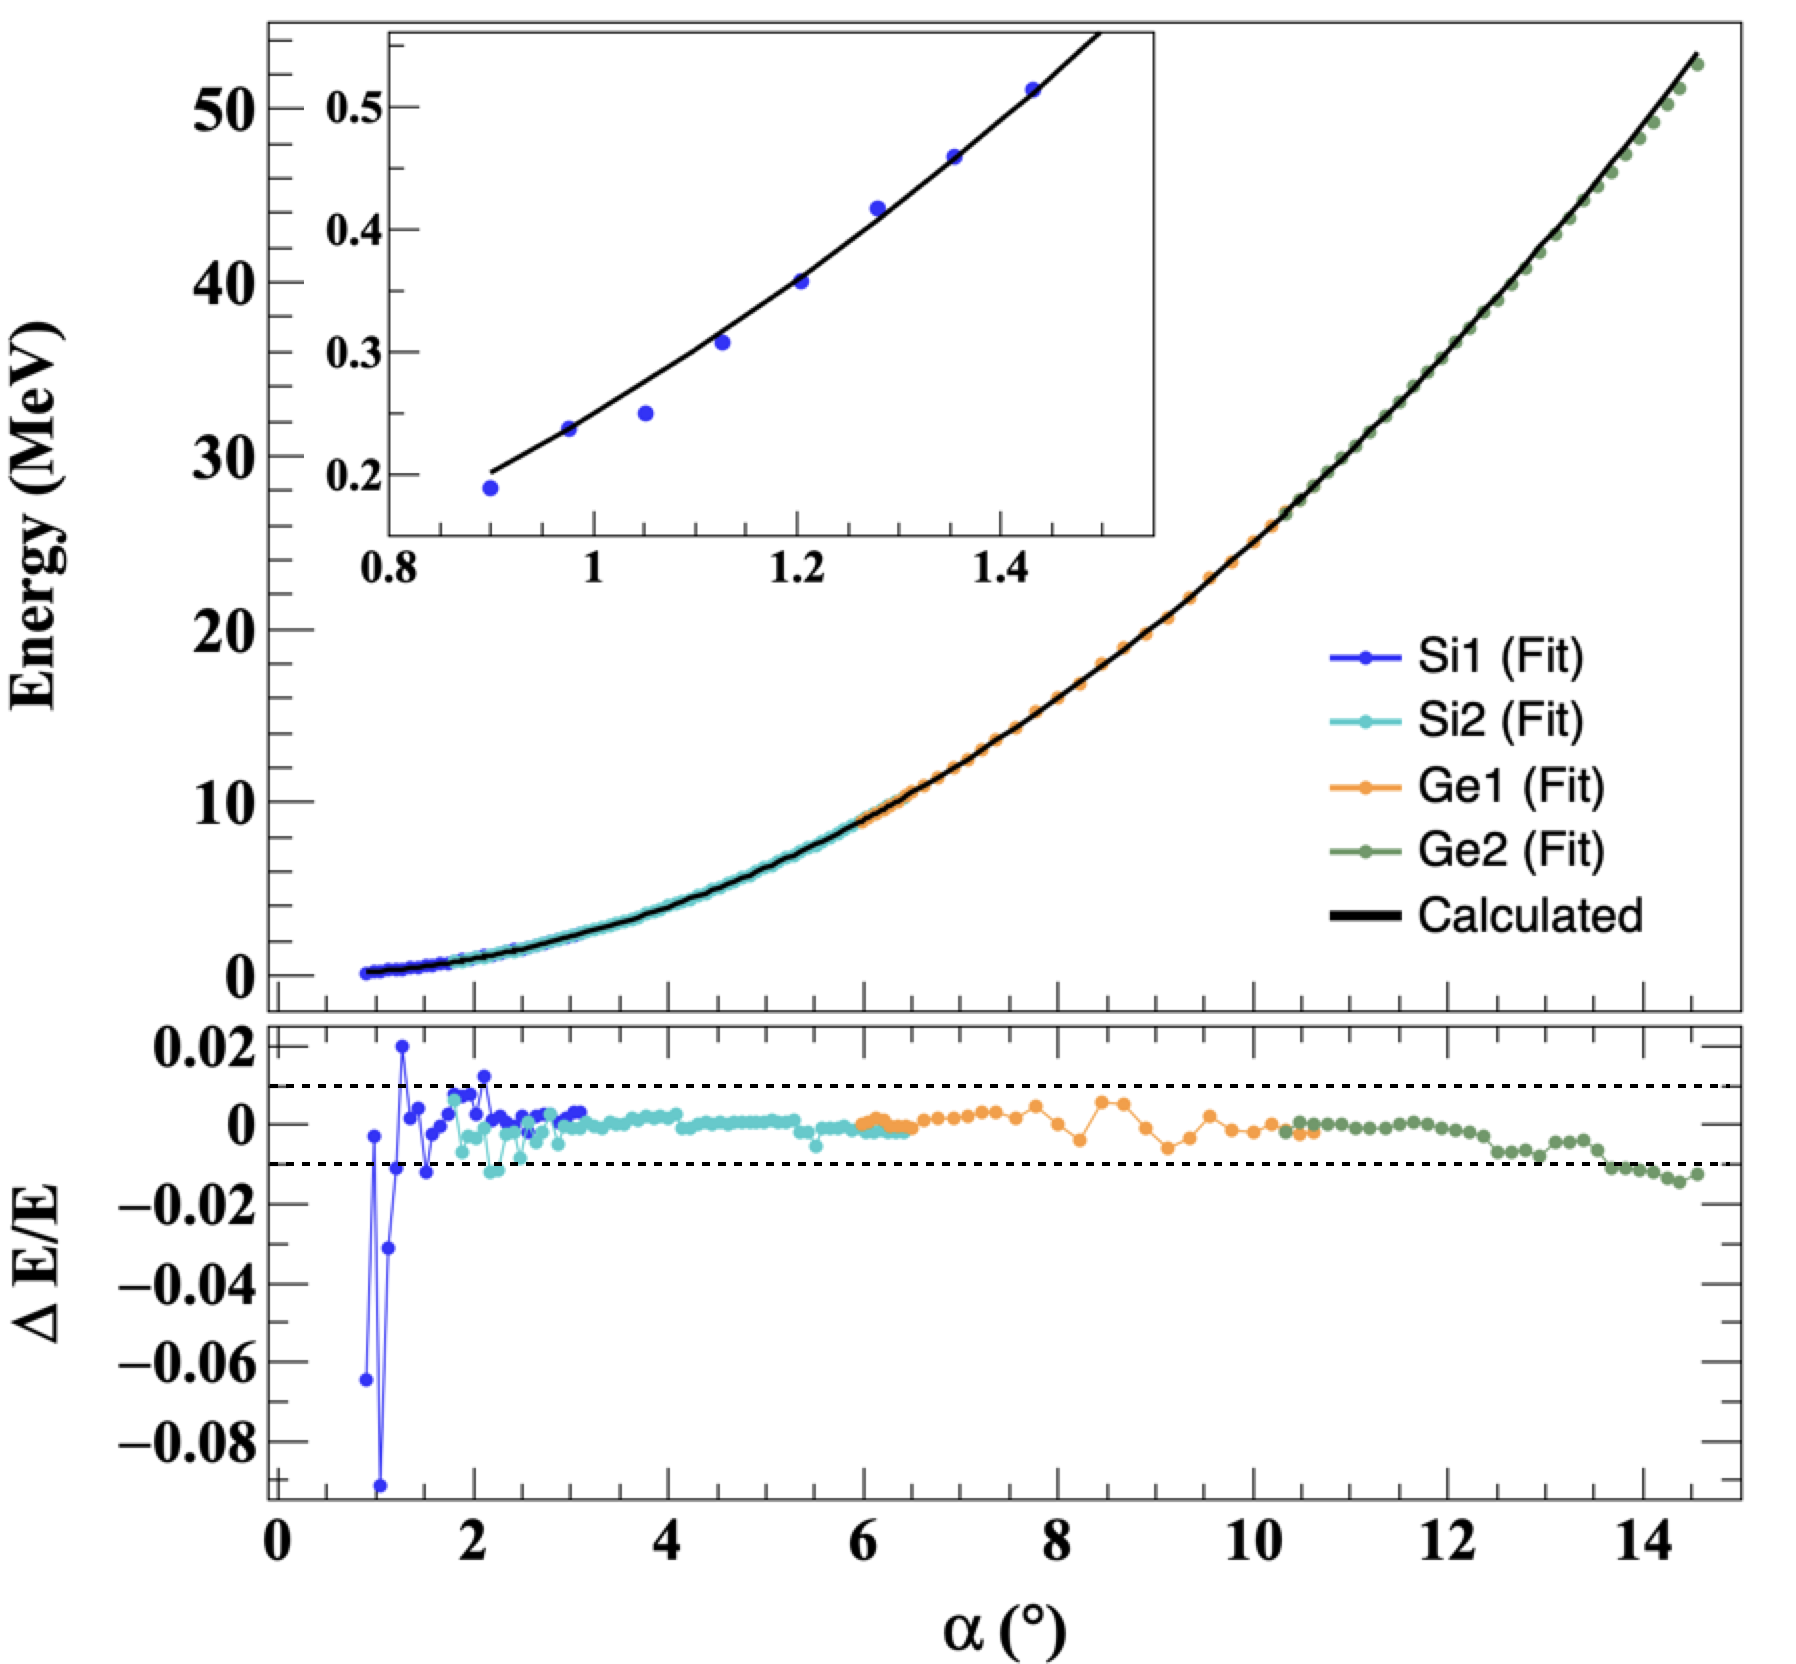
\includegraphics[width=0.45\textwidth]{./e_vs_alpha_combined.png}
  \caption{
    Comparison of the measured (color dots) and the calculated (black line)
    recoil energy on the strip center at different recoil angles. The relative
    difference is drawn in the bottom plot. The results are from $P_{beam} = \SI{2.2}{\momentum}$.}
  \label{fig:measured_vs_calculated}
\end{figure}

\section{Conclusion and Outlook}
\label{sec:conclusion}

The commissioning of the full KOALA setup at COSY, specifically of the new forward detector, is successful.
A strong correlation between the recoil detector and the forward detector is
observed for the covered region of the forward detector.
The idea of using the TOF-E relation of the recoil proton to select elastic
scattering events is verified.
Preliminary analysis shows that lower |t| range can be extended beyond the design
requirement of \SI{0.0008}{\tmom}.

It's found that the finite thickness of the target profile can not be ignored at
very small recoil angles ($\alpha < \SI{1.2}{\degree}$) and it greatly
constraints the lower limit of the $|t|$ measurement.
% The integral thickness of the target profile along the beam-axis is estimated to
% be $\sim$\SI{5.6}{\mm} (FWHM), which is much larger than the design value.
The observed integral thickness of the target profile is larger than the design value.
Since the stochastic cooling was not stable during the beam commissioning, this may be caused by the combined effect of the tilting of the cluster target
beam and the unexpected larger emittance of the COSY beam.
An investigation of the cluster target setup is ongoing and more stable stochastic cooling is required in the future experiment.
Besides, a larger size of the forward scintillators, especially a larger width, is also proposed.

The DAQ operated in a stable condition during the beam commissioning.
% The event synchronization based on the mask gate was used.
However, bias of the trigger efficiency is observed among different sub-detectors.
This is caused by the changing electronic noise level in the COSY environment
and the limited performance of the mask gate based event synchronization.
Due to the self-triggering desgin, different noise triggering levels will change the corresponding trigger efficiency.
Thus, the mask gate in the trigger logic is proposed to be removed and the timestamp-based synchronzation to be used in the future experiment.
A better method for the noise supression is also under investigation.

\bibliographystyle{elsarticle-num}
\bibliography{reference}

\end{document}
